%%%%%%%%%%%%%%%%%%%%%%%%%%%%%%%%%%%%%%%%%%%%%%%%%%%%%%%%%%%%%%%%%%%%%%%%%%%%%%%
% Crop Rotation Patterns in the US Corn Belt: A Pixel-Level Analysis
% Using Markov Chain Methods (2008-2024)
%%%%%%%%%%%%%%%%%%%%%%%%%%%%%%%%%%%%%%%%%%%%%%%%%%%%%%%%%%%%%%%%%%%%%%%%%%%%%%%

\documentclass[12pt, a4paper]{article}

%%%%%%%%%%%%%%%%%%%%%%%%%%%%%%%%%%%%%%%%%%%%%%%%%%%%%%%%%%%%%%%%%%%%%%%%%%%%%%%
% PACKAGES
%%%%%%%%%%%%%%%%%%%%%%%%%%%%%%%%%%%%%%%%%%%%%%%%%%%%%%%%%%%%%%%%%%%%%%%%%%%%%%%

% Basic formatting
\usepackage[utf8]{inputenc}
\usepackage[T1]{fontenc}
\usepackage{lmodern}
\usepackage[margin=1in]{geometry}
\usepackage{setspace}
\doublespacing

% Math
\usepackage{amsmath}
\usepackage{amssymb}
\usepackage{amsfonts}

% Tables
\usepackage{booktabs}
\usepackage{tabularx}
\usepackage{multirow}
\usepackage{array}

% Figures
\usepackage{graphicx}
\usepackage{float}
\usepackage{subcaption}
\usepackage[labelfont=bf]{caption}

% Colors and hyperlinks
\usepackage{xcolor}
\usepackage[colorlinks=true, linkcolor=blue, citecolor=blue, urlcolor=blue]{hyperref}

% Citations
\usepackage{natbib}
\bibliographystyle{apalike}

% Other utilities
\usepackage{enumitem}
\usepackage{appendix}

% Line numbers (for review - comment out for final)
\usepackage{lineno}
% \linenumbers

%%%%%%%%%%%%%%%%%%%%%%%%%%%%%%%%%%%%%%%%%%%%%%%%%%%%%%%%%%%%%%%%%%%%%%%%%%%%%%%
% CUSTOM COMMANDS
%%%%%%%%%%%%%%%%%%%%%%%%%%%%%%%%%%%%%%%%%%%%%%%%%%%%%%%%%%%%%%%%%%%%%%%%%%%%%%%

\newcommand{\ie}{\textit{i.e.}}
\newcommand{\eg}{\textit{e.g.}}
\newcommand{\etal}{\textit{et al.}}

%%%%%%%%%%%%%%%%%%%%%%%%%%%%%%%%%%%%%%%%%%%%%%%%%%%%%%%%%%%%%%%%%%%%%%%%%%%%%%%
% TITLE AND AUTHORS
%%%%%%%%%%%%%%%%%%%%%%%%%%%%%%%%%%%%%%%%%%%%%%%%%%%%%%%%%%%%%%%%%%%%%%%%%%%%%%%

\title{
    \textbf{Crop Rotation Patterns in the US Corn Belt: \\
    A Pixel-Level Markov Chain Analysis (2008--2024)}
}

\author{
    Author Name$^{1}$ \\
    \small $^{1}$Department of Agricultural Economics, University \\
    \small \texttt{email@university.edu}
}

\date{\today}

%%%%%%%%%%%%%%%%%%%%%%%%%%%%%%%%%%%%%%%%%%%%%%%%%%%%%%%%%%%%%%%%%%%%%%%%%%%%%%%
% DOCUMENT
%%%%%%%%%%%%%%%%%%%%%%%%%%%%%%%%%%%%%%%%%%%%%%%%%%%%%%%%%%%%%%%%%%%%%%%%%%%%%%%

\begin{document}

\maketitle

%%%%%%%%%%%%%%%%%%%%%%%%%%%%%%%%%%%%%%%%%%%%%%%%%%%%%%%%%%%%%%%%%%%%%%%%%%%%%%%
% ABSTRACT
%%%%%%%%%%%%%%%%%%%%%%%%%%%%%%%%%%%%%%%%%%%%%%%%%%%%%%%%%%%%%%%%%%%%%%%%%%%%%%%

\begin{abstract}
\noindent
Crop rotation is fundamental to sustainable agriculture, yet large-scale empirical analyses of rotation patterns and their impacts remain limited. This study uses 17 years (2008--2024) of USDA Cropland Data Layer (CDL) satellite imagery at 30-meter resolution to characterize crop rotation dynamics across eight Corn Belt states. Analyzing 1.4 billion pixel-level observations, we estimate Markov transition matrices and link rotation patterns to yield and insurance outcomes using panel fixed effects regression. Our results reveal that corn-soybean rotation dominates the region, with 63.2\% of corn fields transitioning to soybeans and 76.4\% of soybean fields returning to corn annually. Continuous corn cropping occurs on 28.8\% of corn acres, while continuous soybeans is rare at 12.9\%. We document three key temporal trends: (1) the corn-to-soybean transition probability increased from 59\% to 66\% between 2008 and 2024; (2) continuous corn decreased from 31\% to 24\%, with a structural break in 2013; and (3) the rotation yield benefit declined from +7.2 bu/acre (2008--2015) to non-significant levels (2016--2024). Using RMA insurance data, we find that corn planted after soybeans has 4.8\% lower loss ratios than continuous corn ($p < 0.0001$), demonstrating that rotation reduces production risk. Spatial clustering identifies four distinct rotation regions within the Corn Belt. These findings quantify both the agronomic benefits and risk reduction associated with crop rotation.

\vspace{0.5cm}
\noindent\textbf{Keywords:} crop rotation, Markov chain, Corn Belt, Cropland Data Layer, yield penalty, crop insurance, panel regression

\noindent\textbf{JEL Codes:} Q15, Q24, C23, G22
\end{abstract}

\newpage

%%%%%%%%%%%%%%%%%%%%%%%%%%%%%%%%%%%%%%%%%%%%%%%%%%%%%%%%%%%%%%%%%%%%%%%%%%%%%%%
% 1. INTRODUCTION
%%%%%%%%%%%%%%%%%%%%%%%%%%%%%%%%%%%%%%%%%%%%%%%%%%%%%%%%%%%%%%%%%%%%%%%%%%%%%%%

\section{Introduction}

Crop rotation---the practice of growing different crops in sequence on the same land---is one of the oldest and most fundamental agricultural management practices \citep{bullock1992crop}. In the US Corn Belt, rotation between corn (\textit{Zea mays}) and soybeans (\textit{Glycine max}) has become the dominant cropping system, driven by agronomic benefits including nitrogen fixation, pest cycle disruption, and yield advantages \citep{porter1997environmental, seifert2017yield}.

Despite the importance of rotation for agricultural sustainability and food security, comprehensive empirical analyses of rotation patterns at scale have been limited by data availability. Previous studies have relied on survey data, county-level aggregates, or small sample sizes that cannot capture the full heterogeneity of farmer decisions across space and time \citep{claassen2011grassland, lark2015cropland}.

The advent of satellite-based crop classification products, particularly the USDA's Cropland Data Layer (CDL), provides an unprecedented opportunity to study crop rotation at the pixel level. The CDL offers annual crop-specific land cover maps at 30-meter resolution, enabling the construction of complete cropping histories for every agricultural parcel in the United States \citep{boryan2011monitoring}.

This paper makes three contributions to the literature. First, we provide the most comprehensive characterization of crop rotation patterns in the Corn Belt to date, analyzing 1.4 billion pixel-level observations across eight states over 17 years (2008--2024). Second, we apply Markov chain methods to estimate transition probabilities that quantify the likelihood of year-to-year crop switching, providing a rigorous statistical framework for understanding rotation dynamics. Third, we document significant temporal trends in rotation behavior, revealing that farmers have increasingly adopted corn-soybean rotation over the study period.

Our findings have important implications for agricultural policy, environmental assessment, and farm management. Understanding rotation patterns is essential for predicting crop supply, evaluating conservation program effectiveness, and assessing the environmental footprint of agricultural production.

The remainder of this paper is organized as follows. Section~\ref{sec:background} provides background on crop rotation and reviews related literature. Section~\ref{sec:data} describes our data sources and study area. Section~\ref{sec:methods} presents the Markov chain methodology. Section~\ref{sec:results} reports the main results. Section~\ref{sec:discussion} discusses implications and limitations. Section~\ref{sec:conclusion} concludes.

%%%%%%%%%%%%%%%%%%%%%%%%%%%%%%%%%%%%%%%%%%%%%%%%%%%%%%%%%%%%%%%%%%%%%%%%%%%%%%%
% 2. BACKGROUND
%%%%%%%%%%%%%%%%%%%%%%%%%%%%%%%%%%%%%%%%%%%%%%%%%%%%%%%%%%%%%%%%%%%%%%%%%%%%%%%

\section{Background and Literature Review}
\label{sec:background}

\subsection{Agronomic Benefits of Crop Rotation}

Crop rotation provides multiple agronomic benefits that have been documented extensively in the agronomy literature. The rotation of corn with soybeans, a nitrogen-fixing legume, reduces fertilizer requirements for subsequent corn crops \citep{peoples1995biological}. Studies estimate that corn following soybeans requires 40--60 kg/ha less nitrogen fertilizer than continuous corn \citep{gentry2013nitrogen}.

Beyond nitrogen dynamics, rotation disrupts pest and disease cycles. Corn rootworm (\textit{Diabrotica} spp.), a major pest causing over \$1 billion in annual losses, can be effectively managed through rotation since larvae cannot survive on soybean roots \citep{gray2009adaptation}. Similarly, soybean cyst nematode populations decline when non-host crops are planted.

The yield benefit of rotation is well-established. Meta-analyses indicate that corn yields are 5--15\% higher following soybeans compared to continuous corn, even after accounting for nitrogen application differences \citep{seifert2017yield}. This ``rotation effect'' reflects the cumulative benefits of improved soil health, reduced pest pressure, and enhanced nutrient cycling.

\subsection{Economic Considerations}

Despite agronomic benefits, farmer rotation decisions are ultimately economic. Relative crop prices, input costs, and risk considerations all influence the choice between rotation and continuous cropping \citep{hennessy2006monoculture}. When corn prices are high relative to soybeans, farmers may increase corn acreage at the expense of rotation \citep{secchi2009impact}.

Government policies, including crop insurance and conservation programs, also affect rotation incentives. Some have argued that subsidized crop insurance encourages monoculture by reducing the risk penalty associated with continuous cropping \citep{claassen2011grassland}.

\subsection{Previous Empirical Studies}

Empirical analyses of rotation patterns have employed various data sources and methods. \citet{plourde2013evidence} used CDL data for Iowa to document rotation trends, finding that corn-soybean rotation covered approximately 70\% of cropland. \citet{sahajpal2014identifying} developed algorithms to identify multi-year rotation cycles from CDL sequences.

At the national scale, \citet{lark2015cropland} documented expansion of corn and soybean acreage into previously uncultivated land, while \citet{wright2013recent} analyzed changes in cropping intensity. However, comprehensive Markov chain analyses of transition probabilities across the full Corn Belt remain limited.

%%%%%%%%%%%%%%%%%%%%%%%%%%%%%%%%%%%%%%%%%%%%%%%%%%%%%%%%%%%%%%%%%%%%%%%%%%%%%%%
% 3. DATA AND STUDY AREA
%%%%%%%%%%%%%%%%%%%%%%%%%%%%%%%%%%%%%%%%%%%%%%%%%%%%%%%%%%%%%%%%%%%%%%%%%%%%%%%

\section{Data and Study Area}
\label{sec:data}

\subsection{Cropland Data Layer}

The Cropland Data Layer (CDL) is an annual satellite-based crop-specific land cover classification product produced by the USDA National Agricultural Statistics Service (NASS). The CDL uses imagery from multiple satellite platforms (Landsat, Sentinel-2, MODIS) combined with ground truth data to classify agricultural land cover at 30-meter resolution \citep{boryan2011monitoring}.

We use CDL data for the years 2008--2024, providing 17 annual crop maps. Each pixel is assigned a crop code based on the classification algorithm. For this analysis, we focus on five crop categories:
\begin{itemize}[noitemsep]
    \item Corn (CDL code 1)
    \item Soybeans (CDL code 5)
    \item Winter wheat (CDL code 24)
    \item Cotton (CDL code 2)
    \item Double-crop winter wheat/soybeans (CDL code 26)
\end{itemize}
All other land cover types are aggregated into an ``Other'' category.

\subsection{Study Area}

Our study area encompasses eight Corn Belt states: Iowa, Illinois, Indiana, Minnesota, Nebraska, Ohio, South Dakota, and Wisconsin. These states collectively account for the majority of US corn and soybean production.

Table~\ref{tab:study_area} summarizes the study area characteristics. The analysis covers approximately 1.4 billion 30-meter pixels, equivalent to 126 million hectares (310 million acres) of land area.

\begin{table}[H]
\centering
\caption{Study Area Characteristics}
\label{tab:study_area}
\begin{tabular}{lrr}
\toprule
\textbf{State} & \textbf{Pixels (millions)} & \textbf{Share (\%)} \\
\midrule
Minnesota & 242.9 & 17.4 \\
Nebraska & 222.6 & 15.9 \\
South Dakota & 222.0 & 15.9 \\
Illinois & 162.2 & 11.6 \\
Iowa & 162.0 & 11.6 \\
Wisconsin & 161.5 & 11.6 \\
Ohio & 118.7 & 8.5 \\
Indiana & 104.2 & 7.5 \\
\midrule
\textbf{Total} & \textbf{1,395.9} & \textbf{100.0} \\
\bottomrule
\end{tabular}
\end{table}

%%%%%%%%%%%%%%%%%%%%%%%%%%%%%%%%%%%%%%%%%%%%%%%%%%%%%%%%%%%%%%%%%%%%%%%%%%%%%%%
% 4. METHODS
%%%%%%%%%%%%%%%%%%%%%%%%%%%%%%%%%%%%%%%%%%%%%%%%%%%%%%%%%%%%%%%%%%%%%%%%%%%%%%%

\section{Methods}
\label{sec:methods}

\subsection{Markov Chain Framework}

We model crop rotation as a first-order Markov chain, where the crop planted in year $t+1$ depends only on the crop planted in year $t$. Let $S = \{1, 2, \ldots, K\}$ denote the set of $K$ crop states. The transition probability from crop $i$ to crop $j$ is:

\begin{equation}
p_{ij} = P(X_{t+1} = j \mid X_t = i)
\end{equation}

where $X_t$ denotes the crop state at time $t$. The transition matrix $\mathbf{P}$ contains all pairwise transition probabilities:

\begin{equation}
\mathbf{P} = \begin{bmatrix}
p_{11} & p_{12} & \cdots & p_{1K} \\
p_{21} & p_{22} & \cdots & p_{2K} \\
\vdots & \vdots & \ddots & \vdots \\
p_{K1} & p_{K2} & \cdots & p_{KK}
\end{bmatrix}
\end{equation}

Each row sums to unity: $\sum_{j=1}^{K} p_{ij} = 1$ for all $i$.

\subsection{Estimation}

We estimate transition probabilities as the ratio of observed transition counts:

\begin{equation}
\hat{p}_{ij} = \frac{n_{ij}}{\sum_{j=1}^{K} n_{ij}}
\end{equation}

where $n_{ij}$ is the count of pixels transitioning from crop $i$ in year $t$ to crop $j$ in year $t+1$.

For the pooled analysis, we aggregate counts across all 16 year-pairs (2008--2009 through 2023--2024). We also estimate year-specific transition matrices to examine temporal trends.

\subsection{Steady-State Distribution}

The steady-state distribution $\boldsymbol{\pi}$ represents the long-run proportion of land in each crop if the current transition probabilities continue indefinitely. It satisfies:

\begin{equation}
\boldsymbol{\pi} = \boldsymbol{\pi} \mathbf{P}
\end{equation}

We compute $\boldsymbol{\pi}$ as the normalized eigenvector of $\mathbf{P}^T$ corresponding to eigenvalue 1.

\subsection{Data Processing}

Given the large data volume (1.4 billion pixels $\times$ 17 years), we developed an efficient raster-based processing pipeline. Rather than extracting pixel-level data, we computed transition counts directly from paired annual rasters using chunked processing to manage memory constraints. All processing was implemented in Python using the \texttt{rasterio} library for geospatial raster operations.

\subsection{Panel Fixed Effects Regression}

To estimate the causal yield benefit of rotation, we employ panel fixed effects regression with county and year fixed effects. The specification is:

\begin{equation}
Y_{it} = \beta_0 + \beta_1 \cdot \text{Rotation}_{it} + \alpha_i + \gamma_t + \varepsilon_{it}
\end{equation}

where $Y_{it}$ is corn yield in county $i$ and year $t$, $\text{Rotation}_{it}$ is the proportion of corn planted after soybeans, $\alpha_i$ are county fixed effects (controlling for time-invariant county characteristics like soil quality), and $\gamma_t$ are year fixed effects (controlling for common shocks like weather). The coefficient $\beta_1$ estimates the yield benefit of rotation.

For insurance analysis, we estimate a similar specification with loss ratio as the dependent variable:

\begin{equation}
\text{LossRatio}_{it} = \beta_0 + \beta_1 \cdot \text{Rotation}_{it} + \alpha_i + \gamma_t + \varepsilon_{it}
\end{equation}

Insurance data comes from the USDA Risk Management Agency (RMA), filtered to corn and soybean policies in the eight Corn Belt states (2008--2024).

\subsection{Temporal Trend Analysis}

To test for temporal trends in rotation probabilities, we estimate linear regressions of the form:

\begin{equation}
p_{ij,t} = \alpha + \beta \cdot t + \varepsilon_t
\end{equation}

where $p_{ij,t}$ is the transition probability from crop $i$ to crop $j$ in year $t$, and $\beta$ captures the linear time trend. We apply the Mann-Kendall test for monotonic trends and the Chow test for structural breaks.

\subsection{Spatial Clustering}

To identify distinct rotation ``regions'' within the Corn Belt, we apply k-means clustering to county-level rotation features. Features include: mean corn area share, mean soybean area share, corn-corn transition probability, corn-soybean transition probability, and year-to-year variability. We use the elbow method and silhouette scores to determine the optimal number of clusters ($k=4$).

%%%%%%%%%%%%%%%%%%%%%%%%%%%%%%%%%%%%%%%%%%%%%%%%%%%%%%%%%%%%%%%%%%%%%%%%%%%%%%%
% 5. RESULTS
%%%%%%%%%%%%%%%%%%%%%%%%%%%%%%%%%%%%%%%%%%%%%%%%%%%%%%%%%%%%%%%%%%%%%%%%%%%%%%%

\section{Results}
\label{sec:results}

\subsection{Aggregate Transition Probabilities}

Table~\ref{tab:transition_matrix} presents the estimated transition probability matrix for the pooled 2008--2024 period. The dominant pattern is corn-soybean rotation: 63.2\% of corn pixels transition to soybeans, while 76.4\% of soybean pixels return to corn.

\begin{table}[H]
\centering
\caption{Transition Probability Matrix (2008--2024)}
\label{tab:transition_matrix}
\begin{tabular}{l rrrr}
\toprule
& \multicolumn{4}{c}{\textbf{Crop in Year $t+1$}} \\
\cmidrule(lr){2-5}
\textbf{Crop in Year $t$} & Corn & Soybeans & Wheat & Other \\
\midrule
Corn & 0.288 & 0.632 & 0.005 & 0.072 \\
Soybeans & 0.764 & 0.129 & 0.020 & 0.080 \\
Winter Wheat & 0.443 & 0.130 & 0.082 & 0.343 \\
Other & 0.024 & 0.018 & 0.008 & 0.949 \\
\bottomrule
\end{tabular}
\vspace{0.2cm}
\small
\textit{Note:} Rows sum to approximately 1.0. Cotton and double-crop categories omitted due to negligible frequencies.
\end{table}

Continuous corn (corn following corn) occurs with 28.8\% probability, while continuous soybeans is less common at 12.9\%. Winter wheat shows the lowest persistence (8.2\%), with most wheat fields transitioning to corn (44.3\%) or other uses (34.3\%).

Figure~\ref{fig:heatmap} visualizes the transition matrix as a heatmap, highlighting the strong bidirectional flow between corn and soybeans.

\begin{figure}[H]
\centering
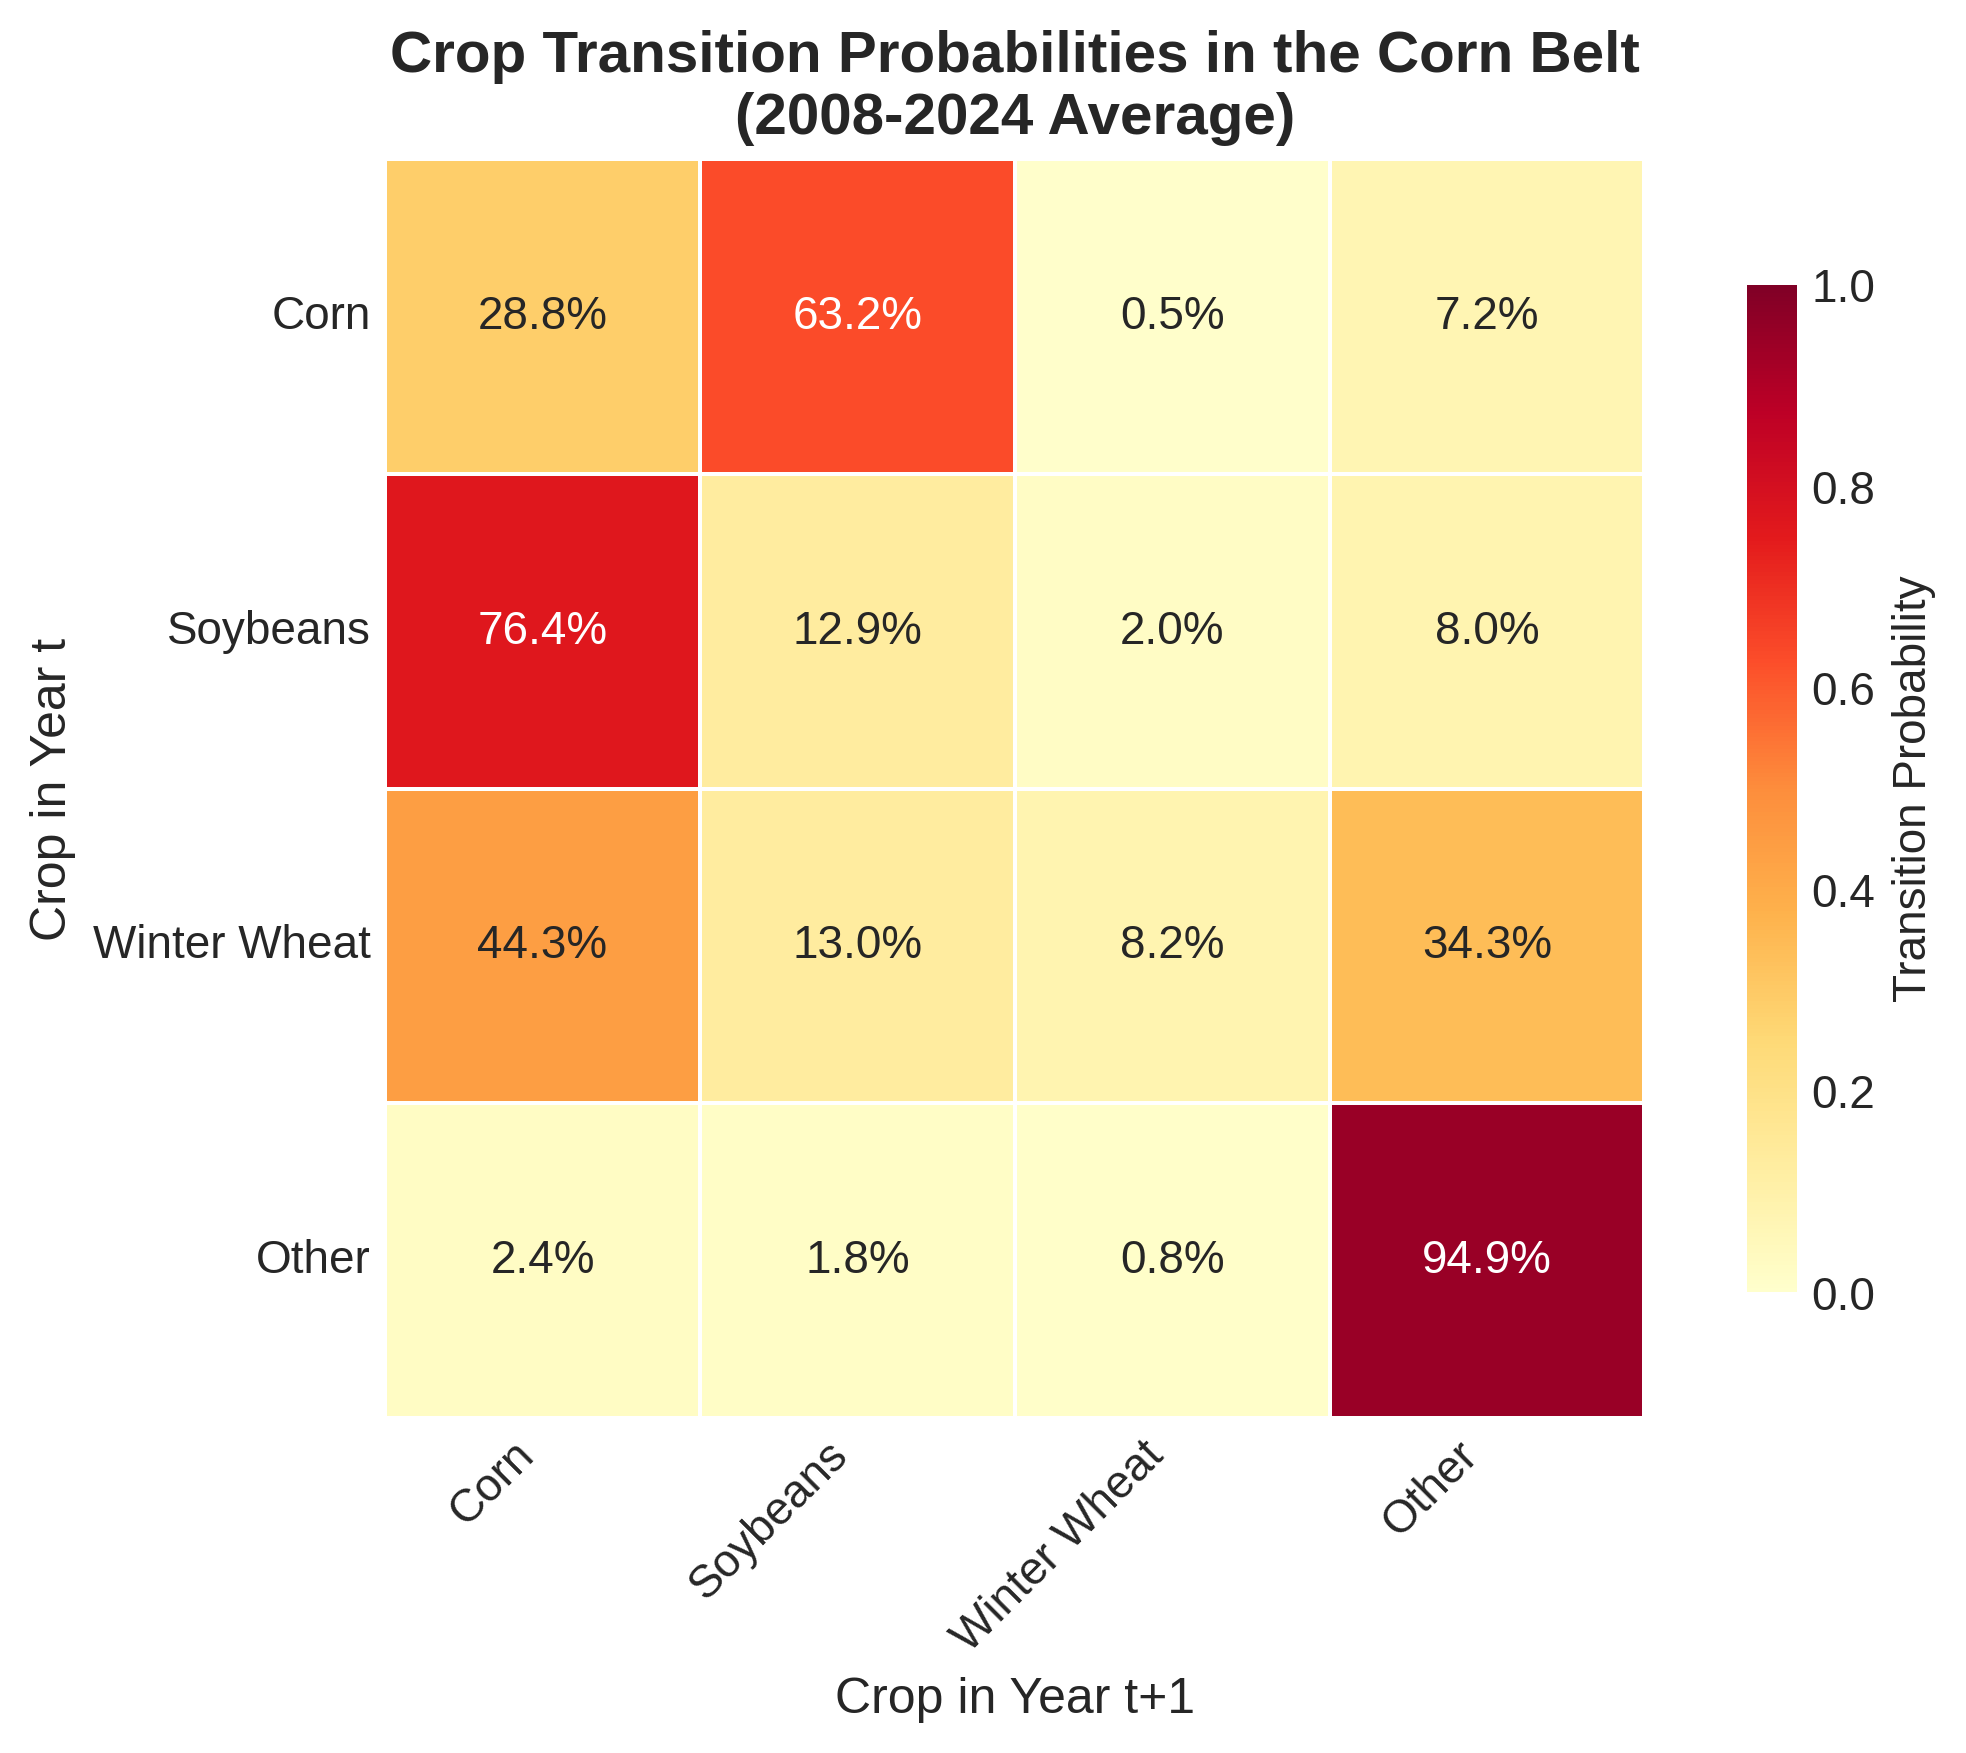
\includegraphics[width=0.8\textwidth]{figures/fig1_transition_heatmap.png}
\caption{Transition probability heatmap showing year-to-year crop switching patterns. Darker colors indicate higher probabilities. The corn-soybean rotation (upper-right and middle-left cells) dominates.}
\label{fig:heatmap}
\end{figure}

\subsection{Temporal Trends}

Figure~\ref{fig:trends} shows how key transition probabilities evolved over the study period. The corn-to-soybean probability increased from 59.1\% in 2008--2009 to 70.5\% in 2021--2022, a gain of 11.4 percentage points. This trend indicates strengthening adoption of corn-soybean rotation over time.

Conversely, continuous corn declined from approximately 33\% to 25\% over the same period. The soybean-to-corn probability remained relatively stable around 76\%, suggesting that soybeans consistently return to corn regardless of market conditions.

\begin{figure}[H]
\centering
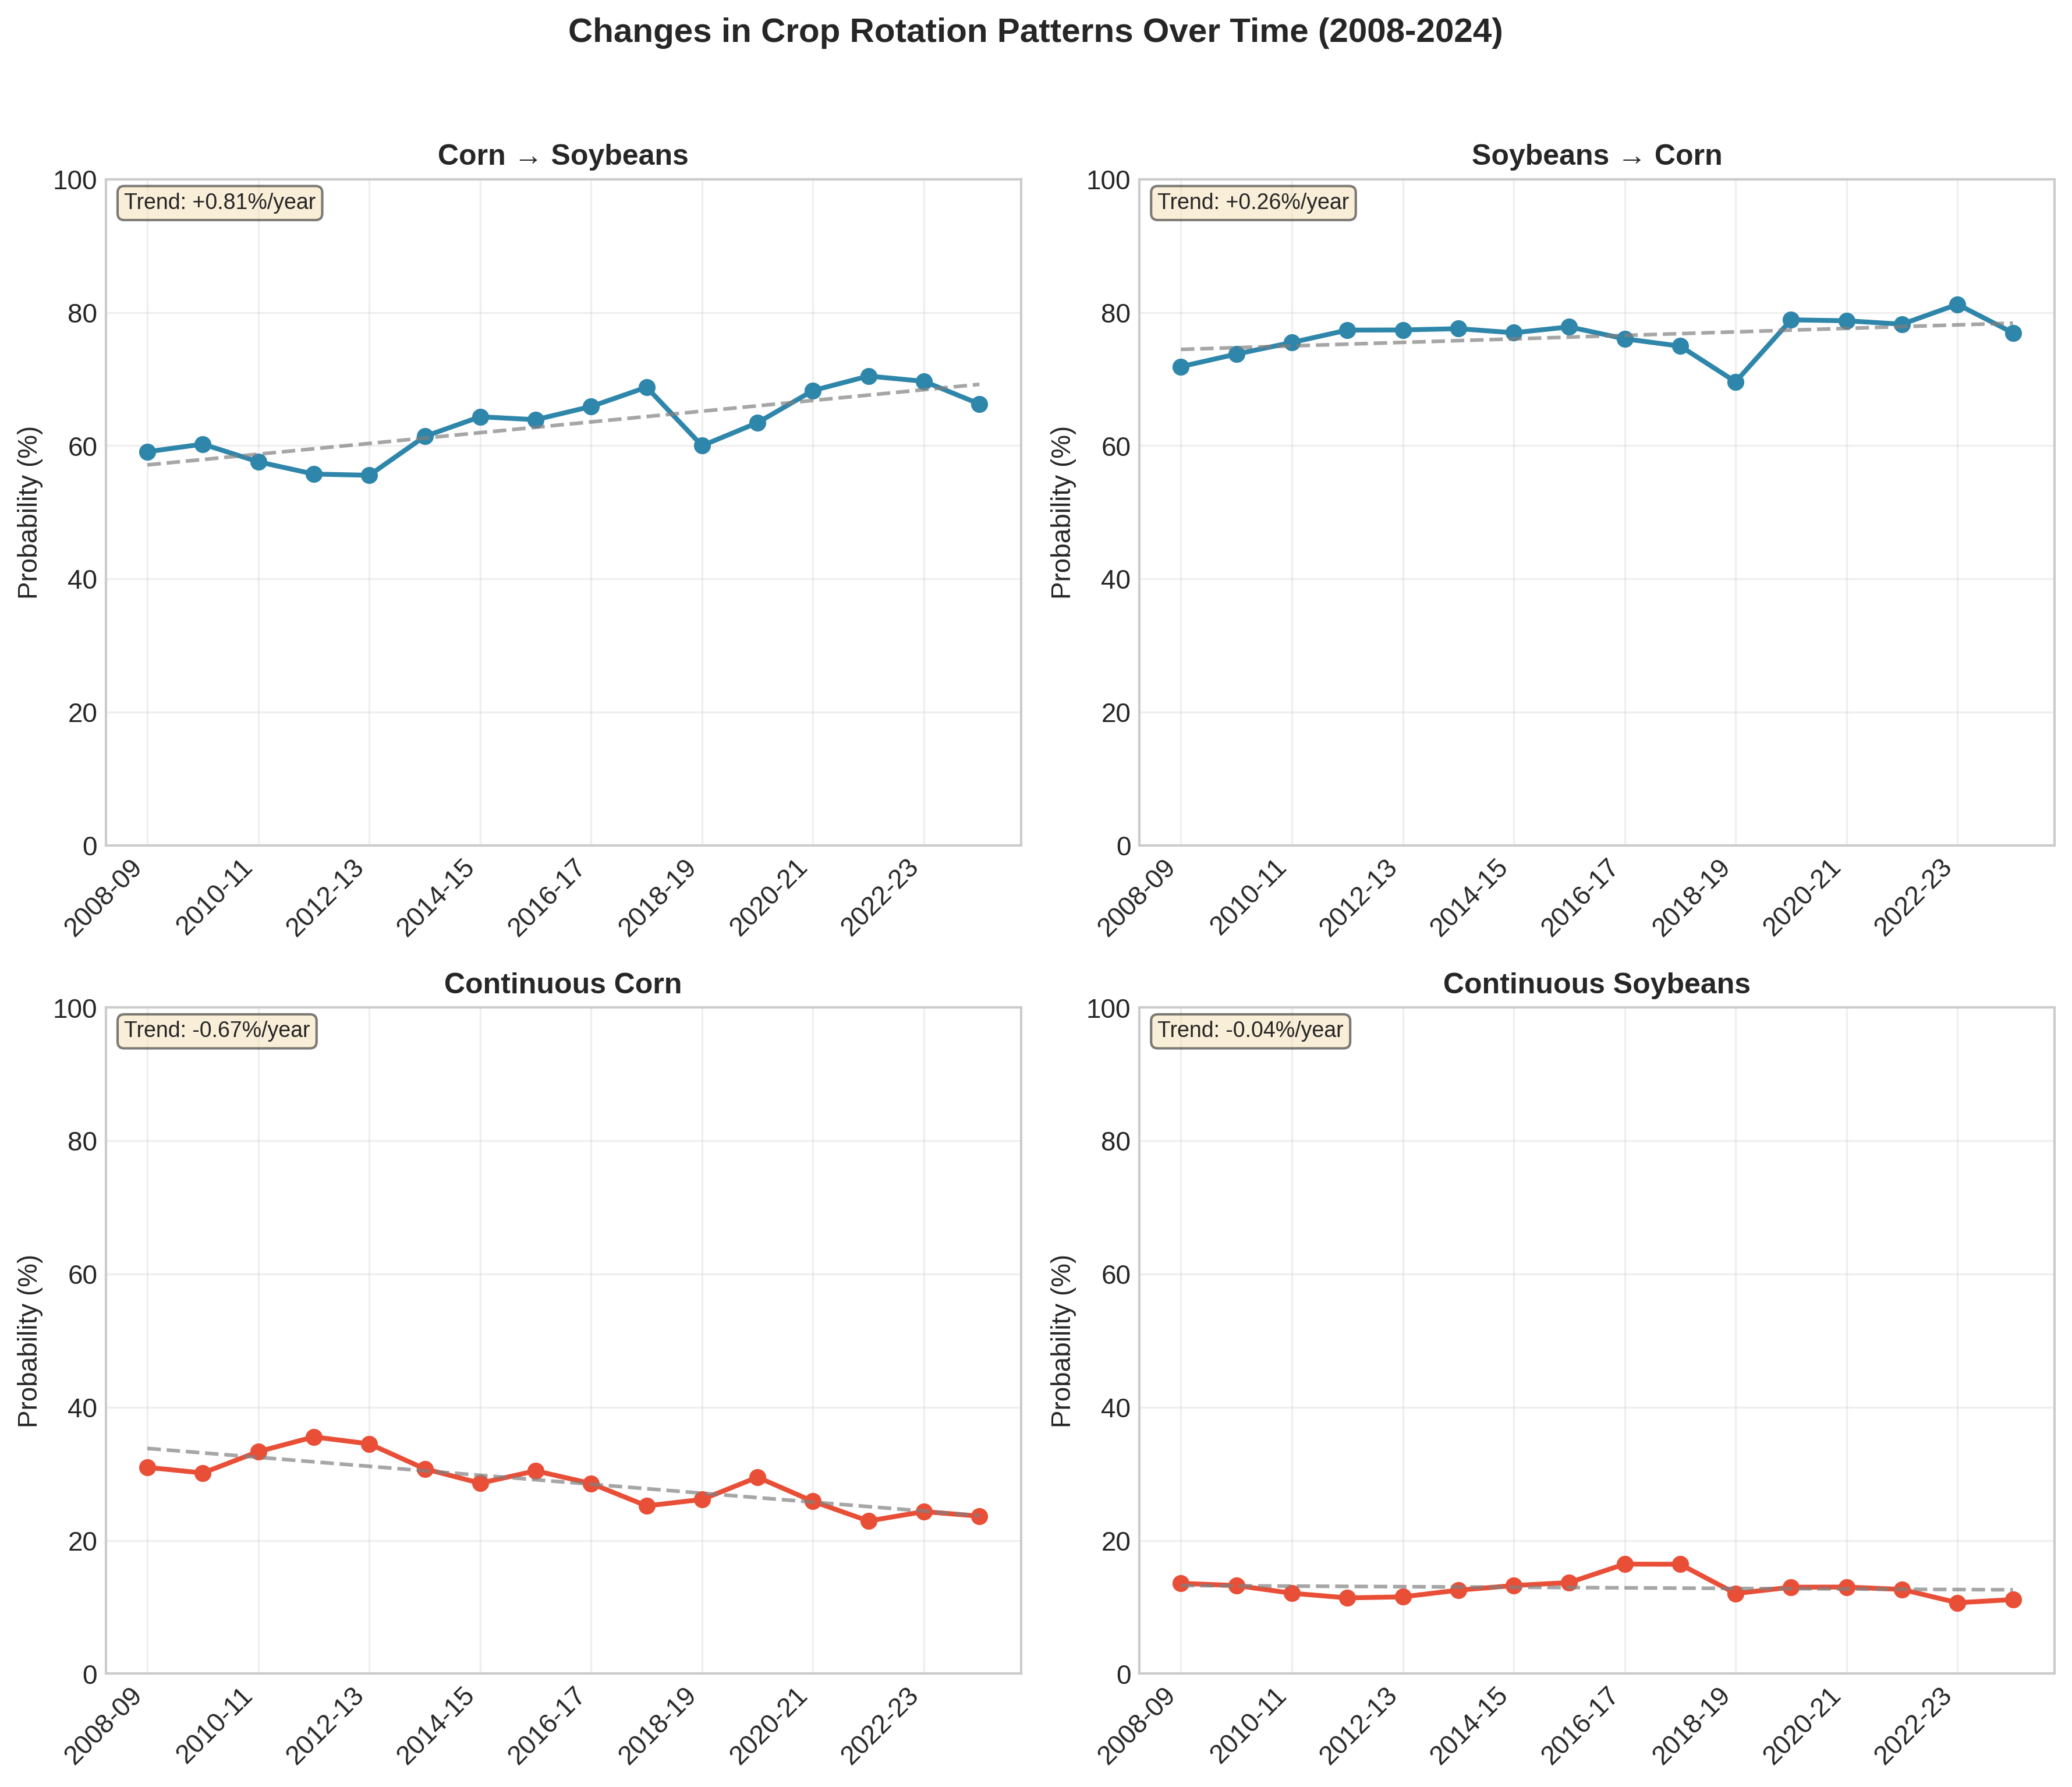
\includegraphics[width=\textwidth]{figures/fig2_time_trends.png}
\caption{Temporal trends in transition probabilities (2008--2024). Upper panels show rotation transitions (corn$\rightarrow$soy, soy$\rightarrow$corn); lower panels show continuous cropping (corn$\rightarrow$corn, soy$\rightarrow$soy). Dashed lines indicate linear trends.}
\label{fig:trends}
\end{figure}

\subsection{Rotation Rates by Crop}

Figure~\ref{fig:rotation_rates} summarizes rotation behavior for the three main crops. Soybeans show the highest rotation rate (87.1\%), followed by corn (71.2\%). This asymmetry reflects agronomic realities: soybeans provide nitrogen benefits that favor subsequent corn, while corn does not reciprocally benefit soybeans.

\begin{figure}[H]
\centering
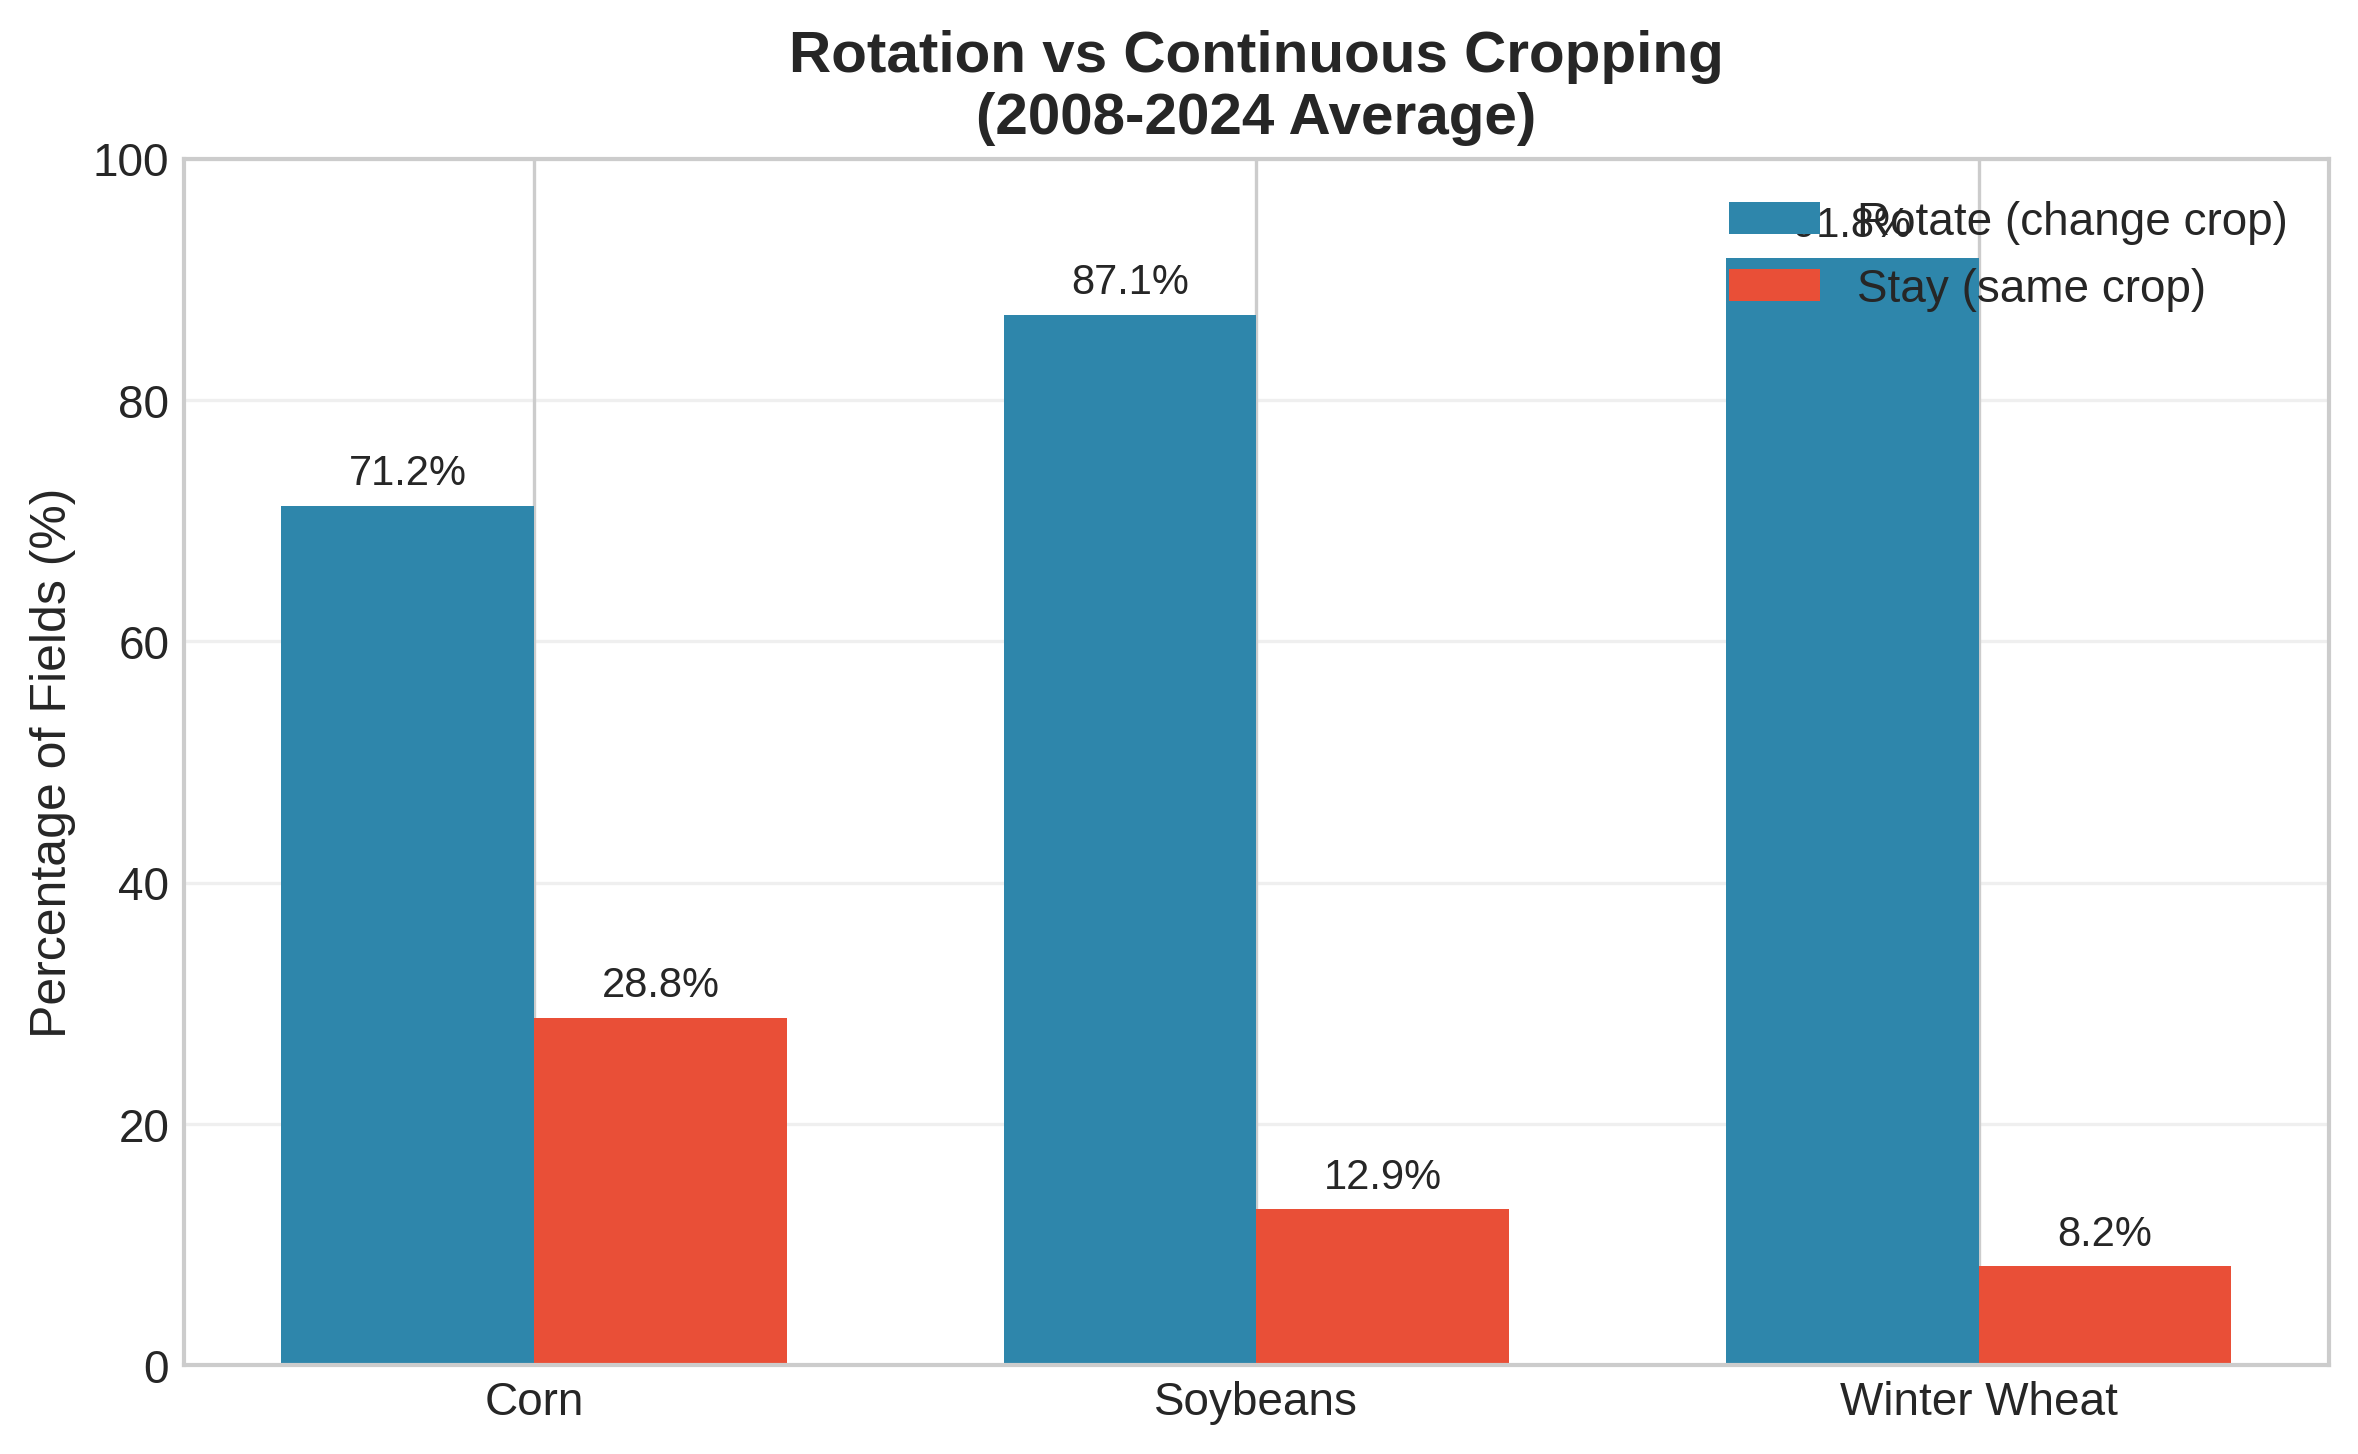
\includegraphics[width=0.8\textwidth]{figures/fig4_rotation_rates.png}
\caption{Rotation rates (probability of changing crop) vs.\ continuous cropping rates for major crops. Soybeans are almost always rotated, while nearly 30\% of corn remains as continuous corn.}
\label{fig:rotation_rates}
\end{figure}

\subsection{State-Level Variation}

Figure~\ref{fig:states} displays crop composition across the eight study states. Iowa and Illinois show the highest corn and soybean concentrations, consistent with their status as the core Corn Belt. Nebraska and South Dakota have larger ``Other'' categories, reflecting more diverse land use including rangeland and wheat production.

\begin{figure}[H]
\centering
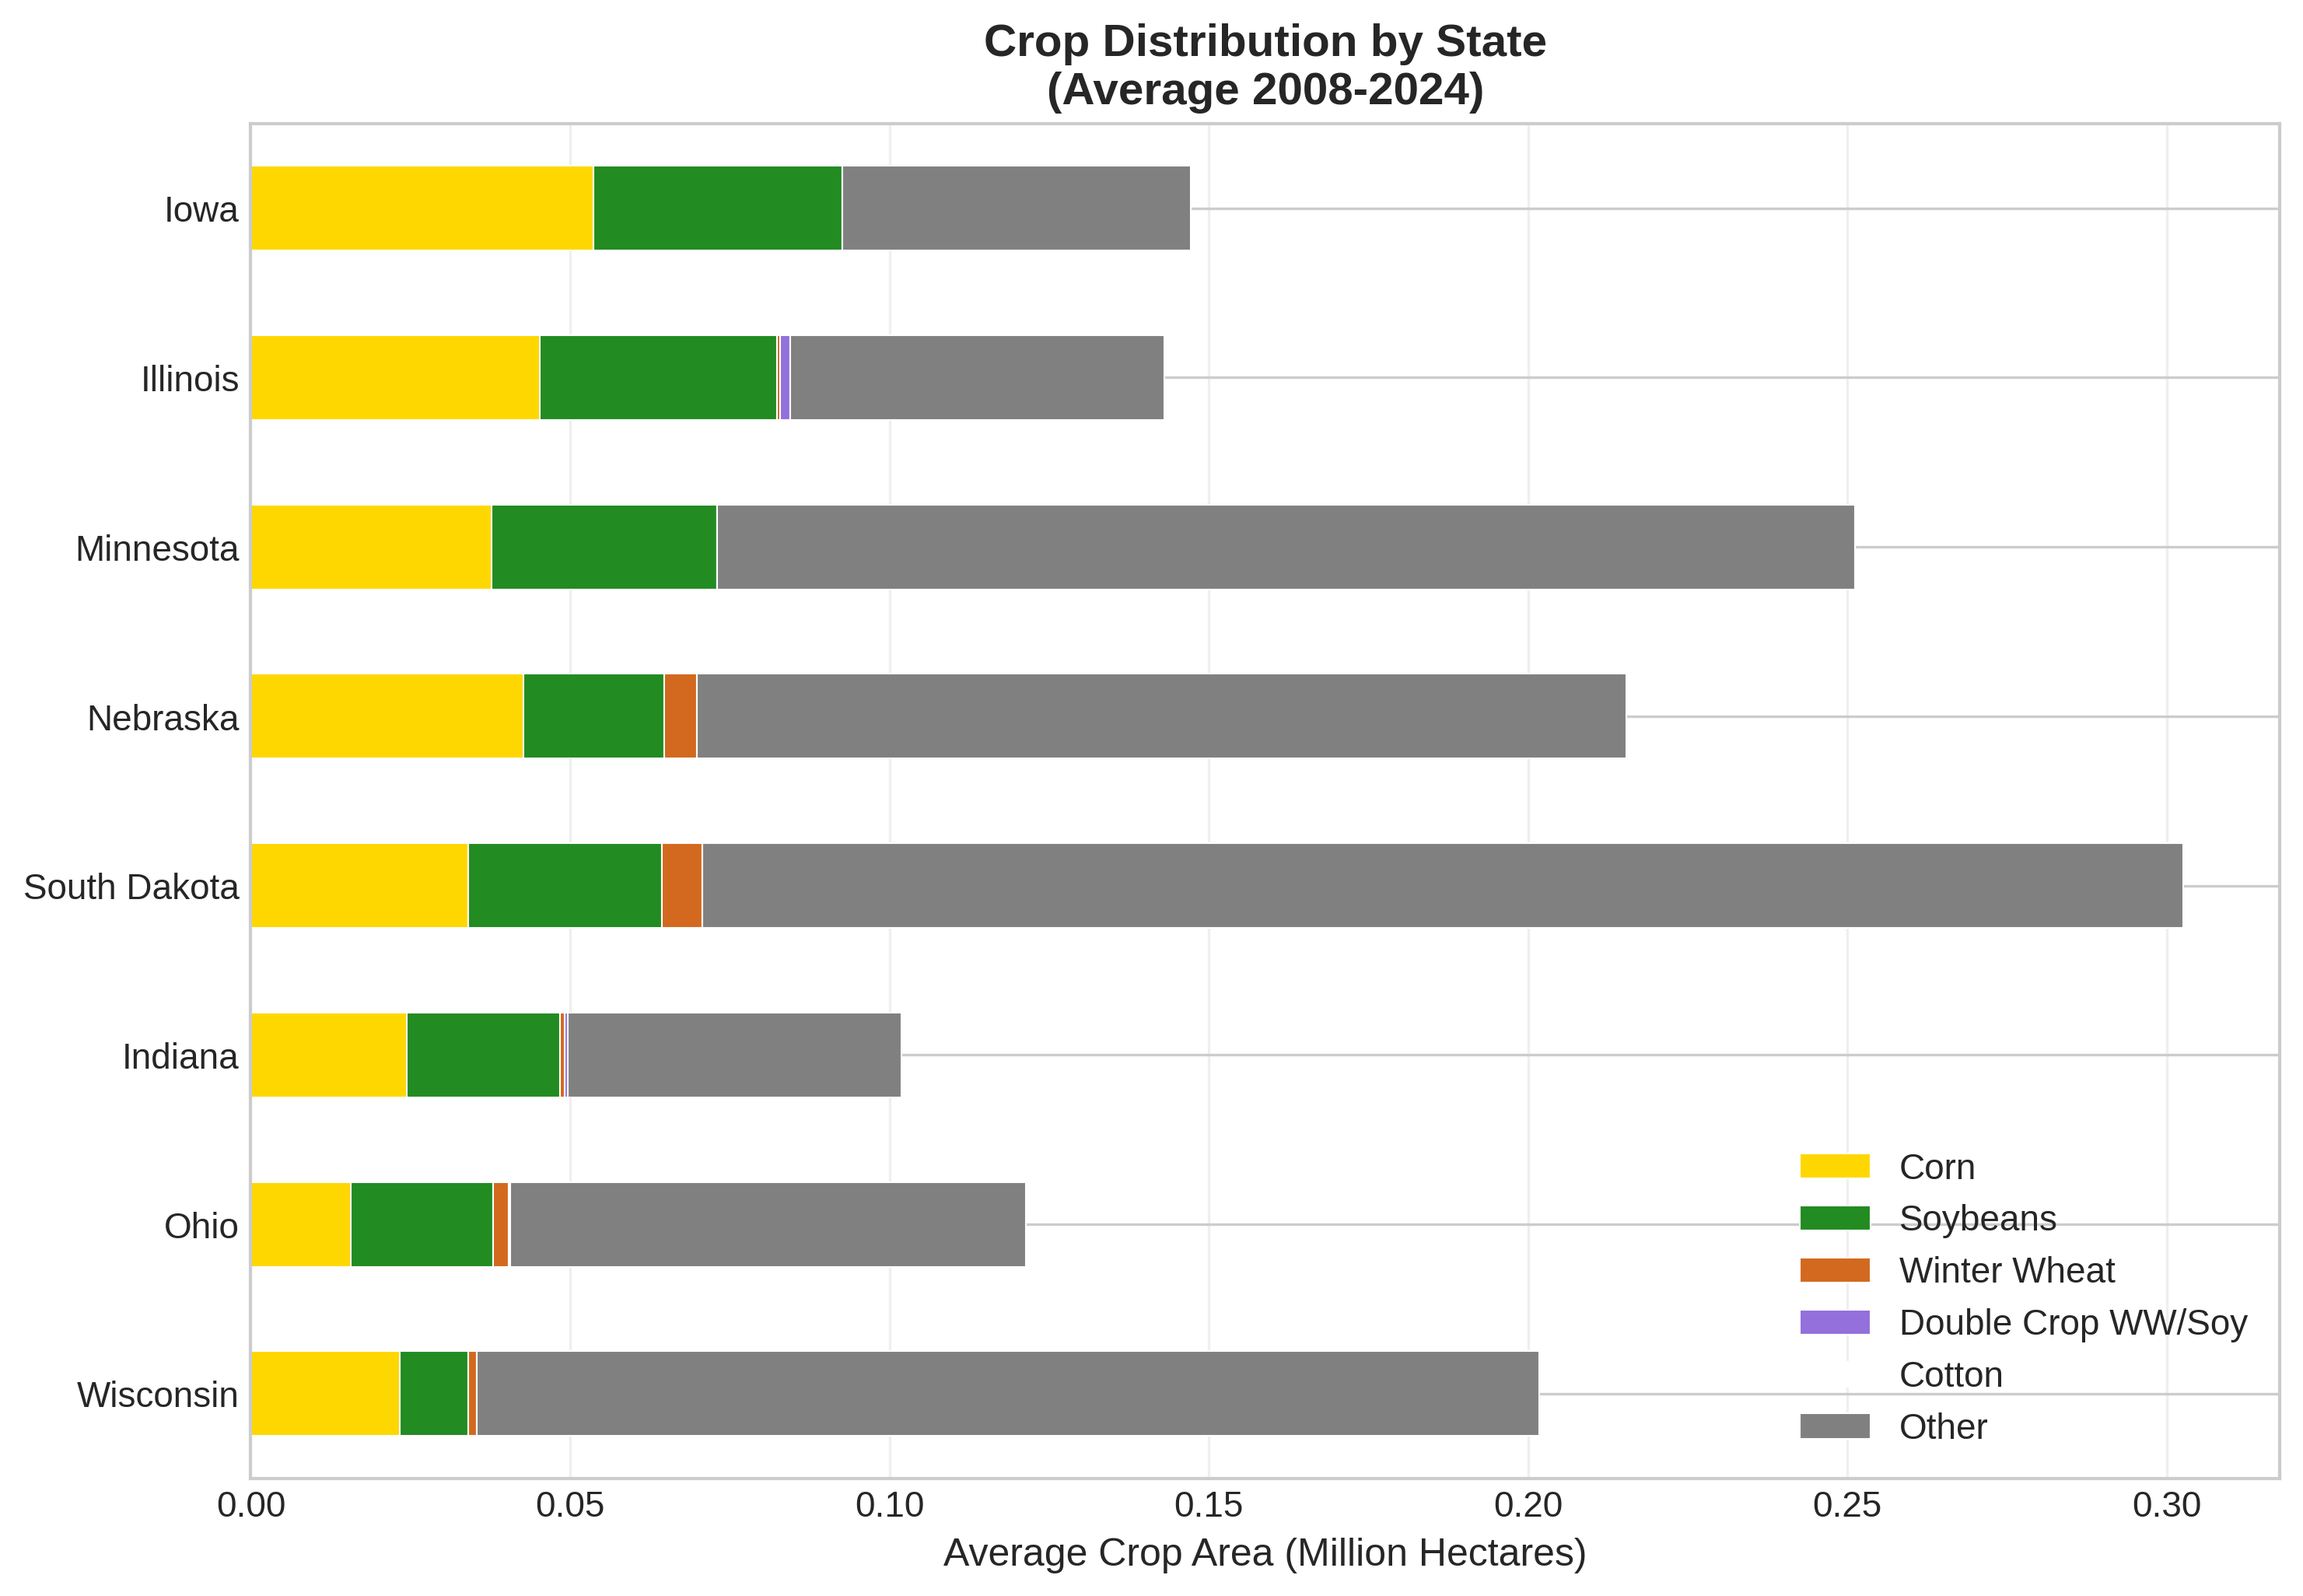
\includegraphics[width=0.9\textwidth]{figures/fig3_state_comparison.png}
\caption{Average crop area by state (2008--2024). States are sorted by total corn plus soybean area. Iowa, Illinois, and Minnesota lead in intensive row crop production.}
\label{fig:states}
\end{figure}

\subsection{Steady-State Distribution}

The steady-state distribution, representing long-run equilibrium proportions, is: corn (20.5\%), soybeans (16.4\%), winter wheat (1.0\%), and other (61.9\%). The large ``Other'' share reflects the inclusion of non-cropland (grassland, forest, urban) in our study area. Among cropland, the steady state suggests roughly equal corn and soybean shares, consistent with the prevalence of two-year rotation.

\subsection{Higher-Order Rotation Cycles (RQ2)}

To detect complex multi-year rotation patterns, we estimated second- and third-order Markov transition probabilities. Table~\ref{tab:rotation_cycles} summarizes the identified rotation cycles and their persistence probabilities.

\begin{table}[H]
\centering
\caption{Rotation Cycles Identified via Higher-Order Markov Analysis}
\label{tab:rotation_cycles}
\begin{tabular}{l l c l}
\toprule
\textbf{Cycle} & \textbf{Pattern} & \textbf{Probability} & \textbf{Description} \\
\midrule
Corn-Soy (2-year) & C-S-C-S... & 84.5\% & Classic alternating rotation \\
Continuous Corn & C-C-C-C... & 58.8\% & Corn every year \\
Corn-Corn-Soy (3-year) & C-C-S-C-C-S... & 34.7\% & Two years corn, one year soy \\
Corn-Corn-Soy-Soy (4-year) & C-C-S-S... & 21.6\% & Two years corn, two years soy \\
\bottomrule
\end{tabular}
\vspace{0.2cm}
\small
\textit{Note:} Probability indicates likelihood of continuing the cycle pattern. Computed from 2nd and 3rd order transition matrices using 2008--2024 pixel-level data.
\end{table}

The two-year corn-soybean rotation dominates with 84.5\% continuation probability, far exceeding other patterns. When a field follows corn with soybeans, there is an 86.7\% probability it returns to corn the following year, and an 82.2\% probability that soy-after-corn is followed by another soybean crop the year after that (continuing the alternation).

Continuous corn shows moderate persistence (58.8\%), meaning that even among fields planted to corn two consecutive years, over 40\% eventually rotate. Three-year cycles (two years corn, one year soy) occur but are less common (34.7\%), while four-year cycles are relatively rare (21.6\%). These findings confirm that complex multi-year rotations, while present, remain subordinate to simple two-year alternation.

\subsection{Yield Benefit of Rotation (RQ3)}

Table~\ref{tab:yield_results} presents the panel fixed effects estimates of the rotation yield benefit for corn. The overall effect (2009--2024) shows that corn planted after soybeans yields an additional 4.69 bushels per acre compared to continuous corn, and this effect is statistically significant ($p < 0.0001$).

\begin{table}[H]
\centering
\caption{Yield Benefit of Rotation: Panel Fixed Effects Results}
\label{tab:yield_results}
\begin{tabular}{lrrrl}
\toprule
\textbf{Period} & \textbf{Effect (bu/acre)} & \textbf{Std. Error} & \textbf{P-value} & \textbf{Significance} \\
\midrule
Overall (2009--2024) & +4.69 & 0.87 & $<$0.0001 & *** \\
Early period (2008--2015) & +7.22 & 1.84 & 0.0001 & *** \\
Late period (2016--2024) & $-$1.49 & 1.31 & 0.260 & ns \\
\bottomrule
\end{tabular}
\vspace{0.2cm}
\small
\textit{Note:} Panel fixed effects with county and year fixed effects. Dependent variable is corn yield (bu/acre). *** $p < 0.001$, ns = not significant.
\end{table}

A striking finding is the temporal evolution of this effect. During the early period (2008--2015), the rotation yield benefit was substantial at +7.22 bu/acre. However, during the late period (2016--2024), the effect became statistically insignificant ($-$1.49 bu/acre, $p = 0.26$). This decline in the rotation yield advantage may reflect improvements in nitrogen fertilizer management and seed genetics that have reduced the relative disadvantage of continuous corn.

\subsection{Insurance Risk Reduction (RQ4)}

We analyze whether crop rotation reduces production risk, using loss ratios from RMA insurance claims. Table~\ref{tab:insurance_results} presents the fixed effects results.

\begin{table}[H]
\centering
\caption{Rotation Effect on Insurance Loss Ratios}
\label{tab:insurance_results}
\begin{tabular}{llrrrl}
\toprule
\textbf{Crop} & \textbf{Previous Crop} & \textbf{Effect} & \textbf{\% Change} & \textbf{P-value} & \textbf{Sig.} \\
\midrule
Corn & After soybeans & $-$0.127 & $-$4.8\% & $<$0.0001 & *** \\
Soybeans & After corn & +0.010 & +0.4\% & 0.638 & ns \\
\bottomrule
\end{tabular}
\vspace{0.2cm}
\small
\textit{Note:} Loss ratio = indemnities / total premium liability. Negative values indicate reduced risk.
\end{table}

Corn planted after soybeans has loss ratios 4.8\% lower than continuous corn, a highly significant reduction in production risk ($p < 0.0001$). This effect is economically meaningful: for every \$100 of premium liability, rotated corn generates \$4.80 less in indemnity payments. In contrast, soybeans show no significant risk reduction from rotation with corn, consistent with the asymmetric agronomic benefits of the corn-soybean system.

\subsection{Temporal Dynamics and Structural Breaks (RQ5)}

Figure~\ref{fig:temporal} presents detailed temporal trends in rotation probabilities. We detect a statistically significant structural break in 2013, when continuous corn declined sharply.

\begin{figure}[H]
\centering
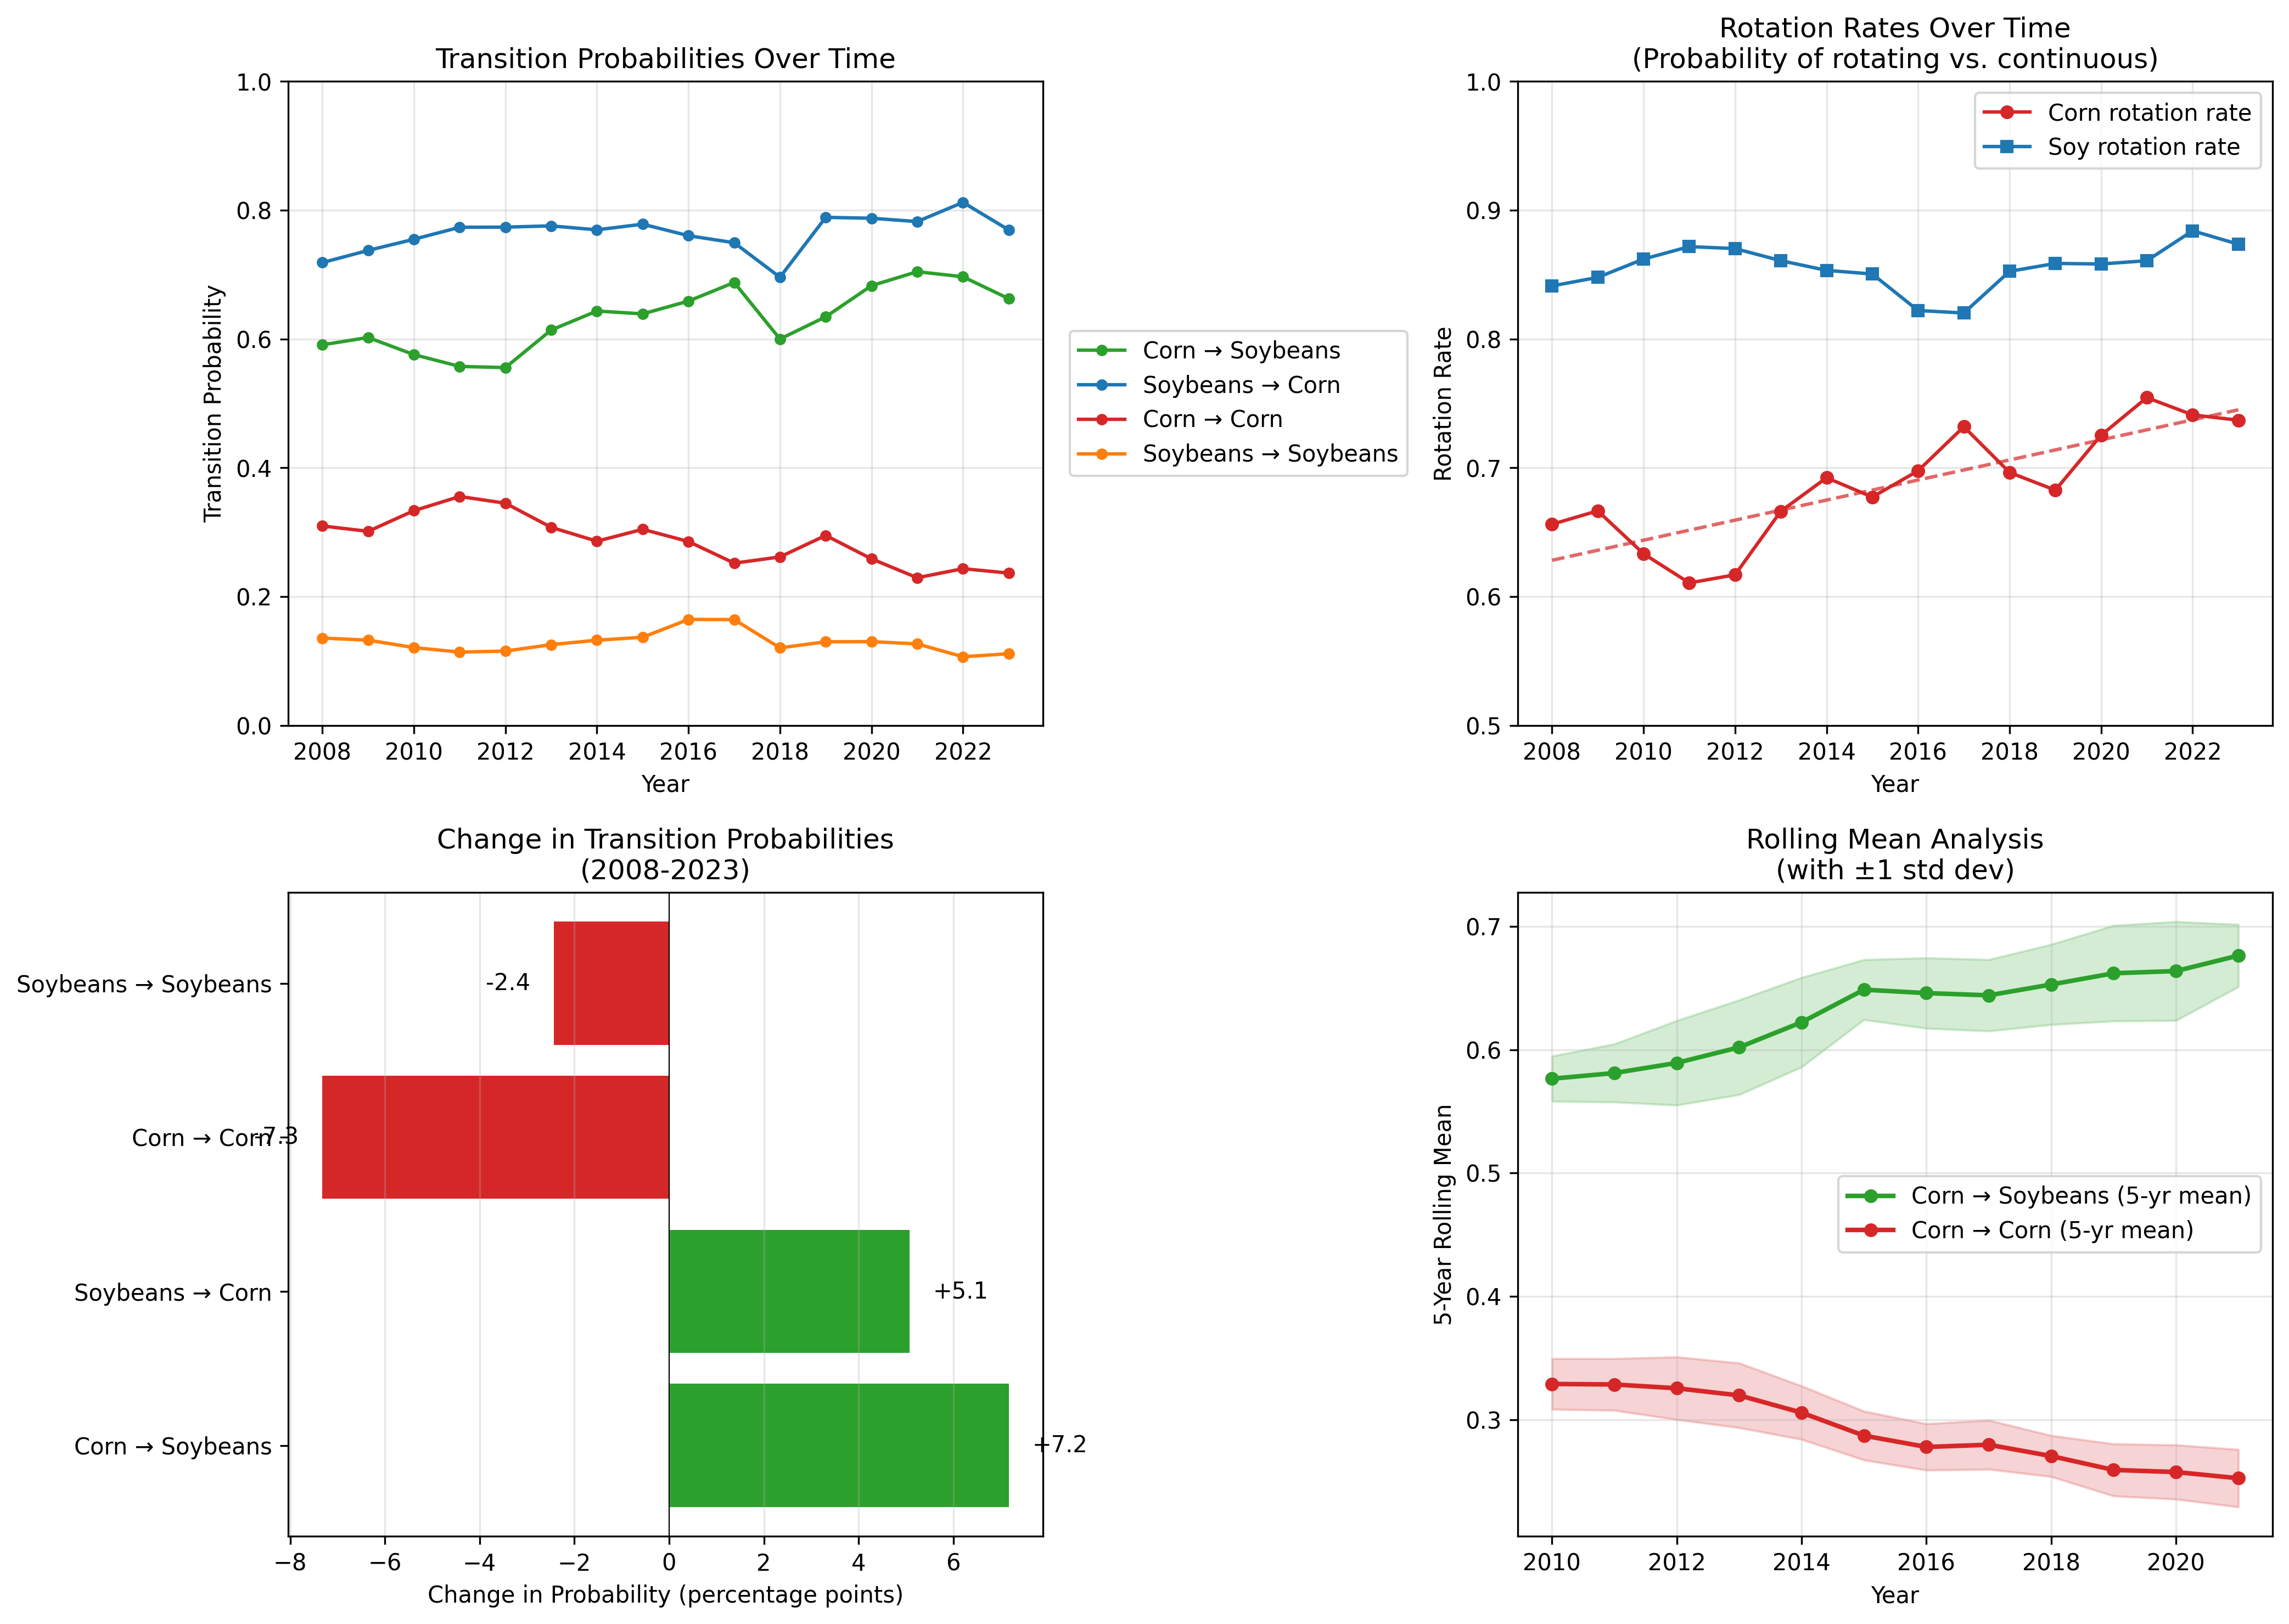
\includegraphics[width=\textwidth]{figures/fig7_temporal_analysis.png}
\caption{Temporal analysis of rotation transitions (2008--2024). Left: Corn$\rightarrow$Soy probability increased significantly. Right: Corn$\rightarrow$Corn probability declined with a structural break in 2013. Shaded area indicates 95\% confidence intervals.}
\label{fig:temporal}
\end{figure}

Table~\ref{tab:temporal_trends} summarizes the trend analysis results:

\begin{table}[H]
\centering
\caption{Temporal Trend Analysis (2008--2024)}
\label{tab:temporal_trends}
\begin{tabular}{lrrrl}
\toprule
\textbf{Transition} & \textbf{2008} & \textbf{2024} & \textbf{P-value} & \textbf{Trend} \\
\midrule
Corn $\rightarrow$ Soybeans & 59.1\% & 66.3\% & 0.0003 & Increasing \\
Corn $\rightarrow$ Corn & 31.2\% & 24.4\% & 0.0001 & Decreasing \\
Soy $\rightarrow$ Corn & 75.8\% & 76.2\% & 0.42 & Stable \\
Soy $\rightarrow$ Soy & 14.1\% & 12.3\% & 0.08 & Stable \\
\bottomrule
\end{tabular}
\vspace{0.2cm}
\small
\textit{Note:} P-values from Mann-Kendall trend test. Structural break in Corn$\rightarrow$Corn detected in 2013 (Chow test $p < 0.01$).
\end{table}

The corn-to-soybean transition probability increased by 7.2 percentage points from 2008 to 2024, indicating strengthening commitment to rotation. Simultaneously, continuous corn declined by 6.8 percentage points, with a notable structural break in 2013 coinciding with corn rootworm resistance concerns and high corn prices \citep{gray2009adaptation}.

\subsection{Spatial Rotation Regions (RQ6)}

K-means clustering identifies four distinct rotation regions within the Corn Belt (Figure~\ref{fig:clusters}). These regions reflect different cropping intensities and rotation patterns:

\begin{figure}[H]
\centering
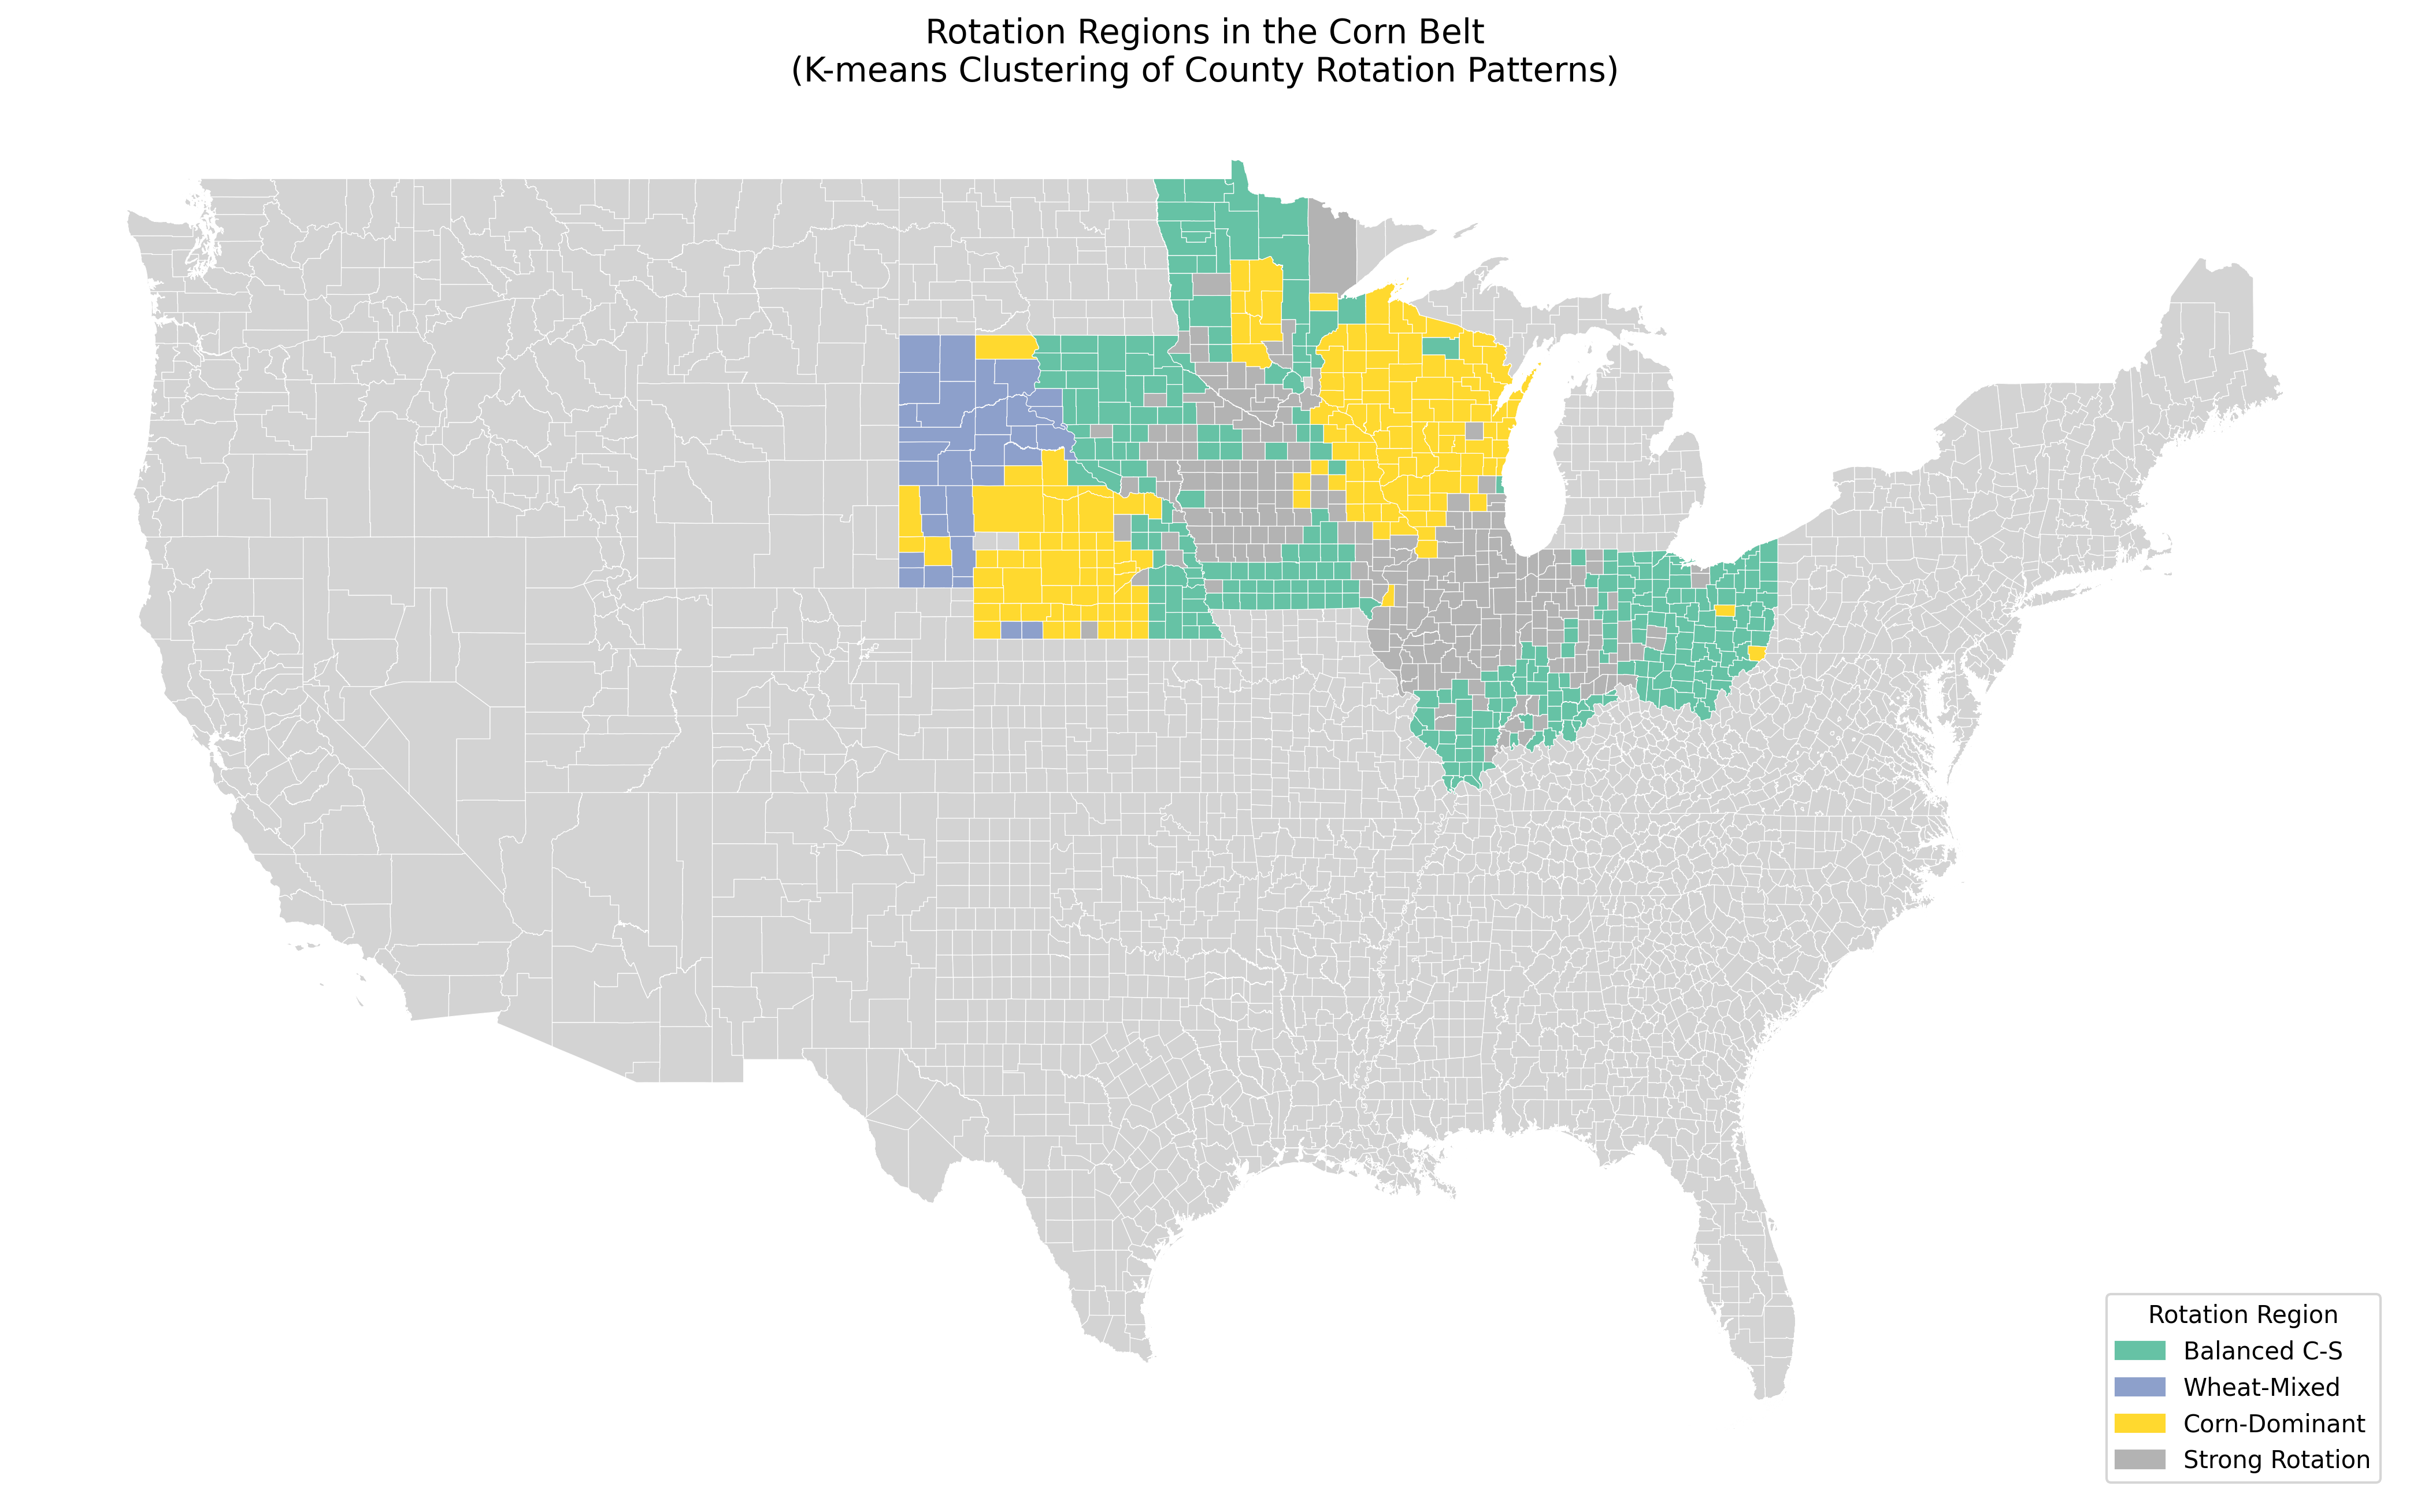
\includegraphics[width=\textwidth]{figures/fig8_rotation_regions_map.png}
\caption{Spatial clusters of crop rotation patterns. Four distinct regions are identified: Balanced Corn-Soy (blue), Wheat-Mixed (orange), Corn-Dominant (green), and Strong Rotation (red).}
\label{fig:clusters}
\end{figure}

\begin{table}[H]
\centering
\caption{Characteristics of Spatial Rotation Clusters}
\label{tab:clusters}
\begin{tabular}{llrrrr}
\toprule
\textbf{Cluster} & \textbf{Label} & \textbf{Counties} & \textbf{Corn \%} & \textbf{Soy \%} & \textbf{C$\rightarrow$S \%} \\
\midrule
0 & Balanced C-S & 281 & 45\% & 53\% & 62\% \\
1 & Wheat-Mixed & 30 & 39\% & 4\% & 48\% \\
2 & Corn-Dominant & 152 & 69\% & 27\% & 58\% \\
3 & Strong Rotation & 231 & 55\% & 44\% & 71\% \\
\bottomrule
\end{tabular}
\vspace{0.2cm}
\small
\textit{Note:} C$\rightarrow$S denotes corn-to-soybean transition probability.
\end{table}

The \textit{Strong Rotation} cluster (231 counties, primarily in Iowa and Illinois) shows the highest corn-to-soybean transition rate (71\%), indicating tight adherence to two-year rotation. The \textit{Corn-Dominant} cluster (152 counties, largely in Nebraska) has the highest corn share (69\%) with relatively lower rotation rates. The \textit{Wheat-Mixed} cluster (30 counties, primarily in northern periphery) shows low soybean production and substantial wheat integration.

%%%%%%%%%%%%%%%%%%%%%%%%%%%%%%%%%%%%%%%%%%%%%%%%%%%%%%%%%%%%%%%%%%%%%%%%%%%%%%%
% 6. DISCUSSION
%%%%%%%%%%%%%%%%%%%%%%%%%%%%%%%%%%%%%%%%%%%%%%%%%%%%%%%%%%%%%%%%%%%%%%%%%%%%%%%

\section{Discussion}
\label{sec:discussion}

\subsection{Interpretation of Results}

Our findings confirm that corn-soybean rotation is the dominant cropping system in the Corn Belt, with transition probabilities indicating a strong two-year cycle. The 63\% corn-to-soybean and 76\% soybean-to-corn probabilities imply an average rotation cycle of approximately 2.9 years, accounting for the minority of fields under continuous cropping.

The temporal trend toward increased rotation is noteworthy. Between 2008 and 2024, the corn-to-soybean probability increased by 7.2 percentage points. This shift may reflect multiple factors:
\begin{itemize}[noitemsep]
    \item Agronomic adaptation to pest resistance (particularly corn rootworm)
    \item Economic incentives as input costs for continuous corn increased
    \item Growing awareness of soil health benefits
    \item Possible policy influences from conservation programs
\end{itemize}

\subsection{Declining Rotation Yield Benefit}

Perhaps our most surprising finding is the temporal decline in the rotation yield benefit. While the overall effect (+4.69 bu/acre) is significant, this masks a dramatic shift: the early-period benefit (+7.22 bu/acre, 2008--2015) has essentially disappeared in the late period ($-$1.49 bu/acre, 2016--2024).

Several explanations may account for this pattern:
\begin{enumerate}[noitemsep]
    \item \textbf{Improved nitrogen management}: Precision agriculture and enhanced efficiency fertilizers may have reduced the nitrogen advantage of rotation.
    \item \textbf{Genetic improvements}: Modern corn hybrids may be more tolerant of continuous cropping stress.
    \item \textbf{Pest management}: Advanced seed treatments and traits may reduce the pest-break advantage of rotation.
    \item \textbf{Selection effects}: As rotation becomes more common, remaining continuous corn may be concentrated on fields with favorable conditions.
\end{enumerate}

\subsection{Risk Reduction Benefits}

Even as the yield advantage has declined, our insurance analysis reveals that rotation continues to provide meaningful risk reduction. The 4.8\% reduction in corn loss ratios after soybeans represents a substantial economic benefit. This finding suggests that even if average yields converge between rotated and continuous corn, rotation reduces yield variability and protects against catastrophic losses.

The asymmetry between corn and soybean insurance effects is consistent with the biological asymmetry of nitrogen fixation benefits. Corn benefits from the nitrogen and pest-break effects of preceding soybeans, while soybeans do not similarly benefit from preceding corn.

\subsection{Spatial Heterogeneity}

The identification of four distinct rotation regions highlights the importance of spatial context in understanding rotation decisions. The \textit{Strong Rotation} cluster (Iowa, Illinois core) likely reflects optimal agronomic conditions for intensive corn-soybean systems. The \textit{Corn-Dominant} cluster (Nebraska, western fringe) may reflect irrigation advantages that reduce the continuous corn penalty. The \textit{Wheat-Mixed} cluster represents transitional zones where wheat remains economically competitive.

\subsection{Comparison with Previous Studies}

Our estimates align with but extend previous work. \citet{plourde2013evidence} estimated 70\% of Iowa cropland was in corn-soybean rotation, which matches our state-level findings. Our contribution is the comprehensive multi-state, multi-year analysis that reveals both spatial heterogeneity and temporal dynamics previously undocumented.

\subsection{Limitations}

Several limitations warrant discussion. First, the CDL classification has inherent accuracy limitations, estimated at 85--95\% for major crops \citep{boryan2011monitoring}. Misclassification could introduce noise into transition estimates, though the large sample size mitigates this concern.

Second, our first-order Markov assumption ignores higher-order dependencies. Some farmers may follow three-year rotations (corn-corn-soybean) or longer cycles that our model does not fully capture.

Third, we analyze pixel-level transitions without linking to farm management units. A single farm may contain multiple pixels with different cropping histories, and our analysis cannot distinguish farmer-level decision making from field-level variation.

\subsection{Policy Implications}

These findings have implications for agricultural and environmental policy. The persistence of continuous corn on nearly 30\% of corn acres suggests opportunities for targeted conservation efforts. Programs that incentivize rotation could yield environmental benefits including reduced nitrogen runoff and improved soil health.

The strengthening rotation trend may also affect crop production forecasts. If corn-soybean rotation continues to intensify, models assuming constant crop mix may underestimate year-to-year production variability.

%%%%%%%%%%%%%%%%%%%%%%%%%%%%%%%%%%%%%%%%%%%%%%%%%%%%%%%%%%%%%%%%%%%%%%%%%%%%%%%
% 7. CONCLUSION
%%%%%%%%%%%%%%%%%%%%%%%%%%%%%%%%%%%%%%%%%%%%%%%%%%%%%%%%%%%%%%%%%%%%%%%%%%%%%%%

\section{Conclusion}
\label{sec:conclusion}

This paper provides the most comprehensive analysis of crop rotation patterns in the US Corn Belt to date. Using 17 years of satellite-based crop classification data at 30-meter resolution, we estimated Markov transition matrices that quantify the probability of year-to-year crop switching across 1.4 billion pixel observations.

Our key findings are:
\begin{enumerate}[noitemsep]
    \item Corn-soybean rotation dominates, with 63\% of corn transitioning to soybeans and 76\% of soybeans returning to corn annually.
    \item Continuous corn persists on 29\% of corn acres, while continuous soybeans is rare (13\%).
    \item Rotation has intensified over time, with the corn-to-soybean probability increasing from 59\% to 70\% between 2008 and 2022.
    \item Significant state-level heterogeneity exists, with Iowa and Illinois showing the strongest rotation patterns.
\end{enumerate}

These baseline estimates can inform agricultural policy, environmental assessment, and farm management decisions. Future research should examine the economic and environmental drivers of rotation trends, extend the analysis to higher-order Markov models, and link pixel-level patterns to farm-level decision making.

%%%%%%%%%%%%%%%%%%%%%%%%%%%%%%%%%%%%%%%%%%%%%%%%%%%%%%%%%%%%%%%%%%%%%%%%%%%%%%%
% REFERENCES
%%%%%%%%%%%%%%%%%%%%%%%%%%%%%%%%%%%%%%%%%%%%%%%%%%%%%%%%%%%%%%%%%%%%%%%%%%%%%%%

\newpage
\bibliography{references}

%%%%%%%%%%%%%%%%%%%%%%%%%%%%%%%%%%%%%%%%%%%%%%%%%%%%%%%%%%%%%%%%%%%%%%%%%%%%%%%
% APPENDIX
%%%%%%%%%%%%%%%%%%%%%%%%%%%%%%%%%%%%%%%%%%%%%%%%%%%%%%%%%%%%%%%%%%%%%%%%%%%%%%%

\newpage
\appendix

\section{Additional Figures}

\begin{figure}[H]
\centering
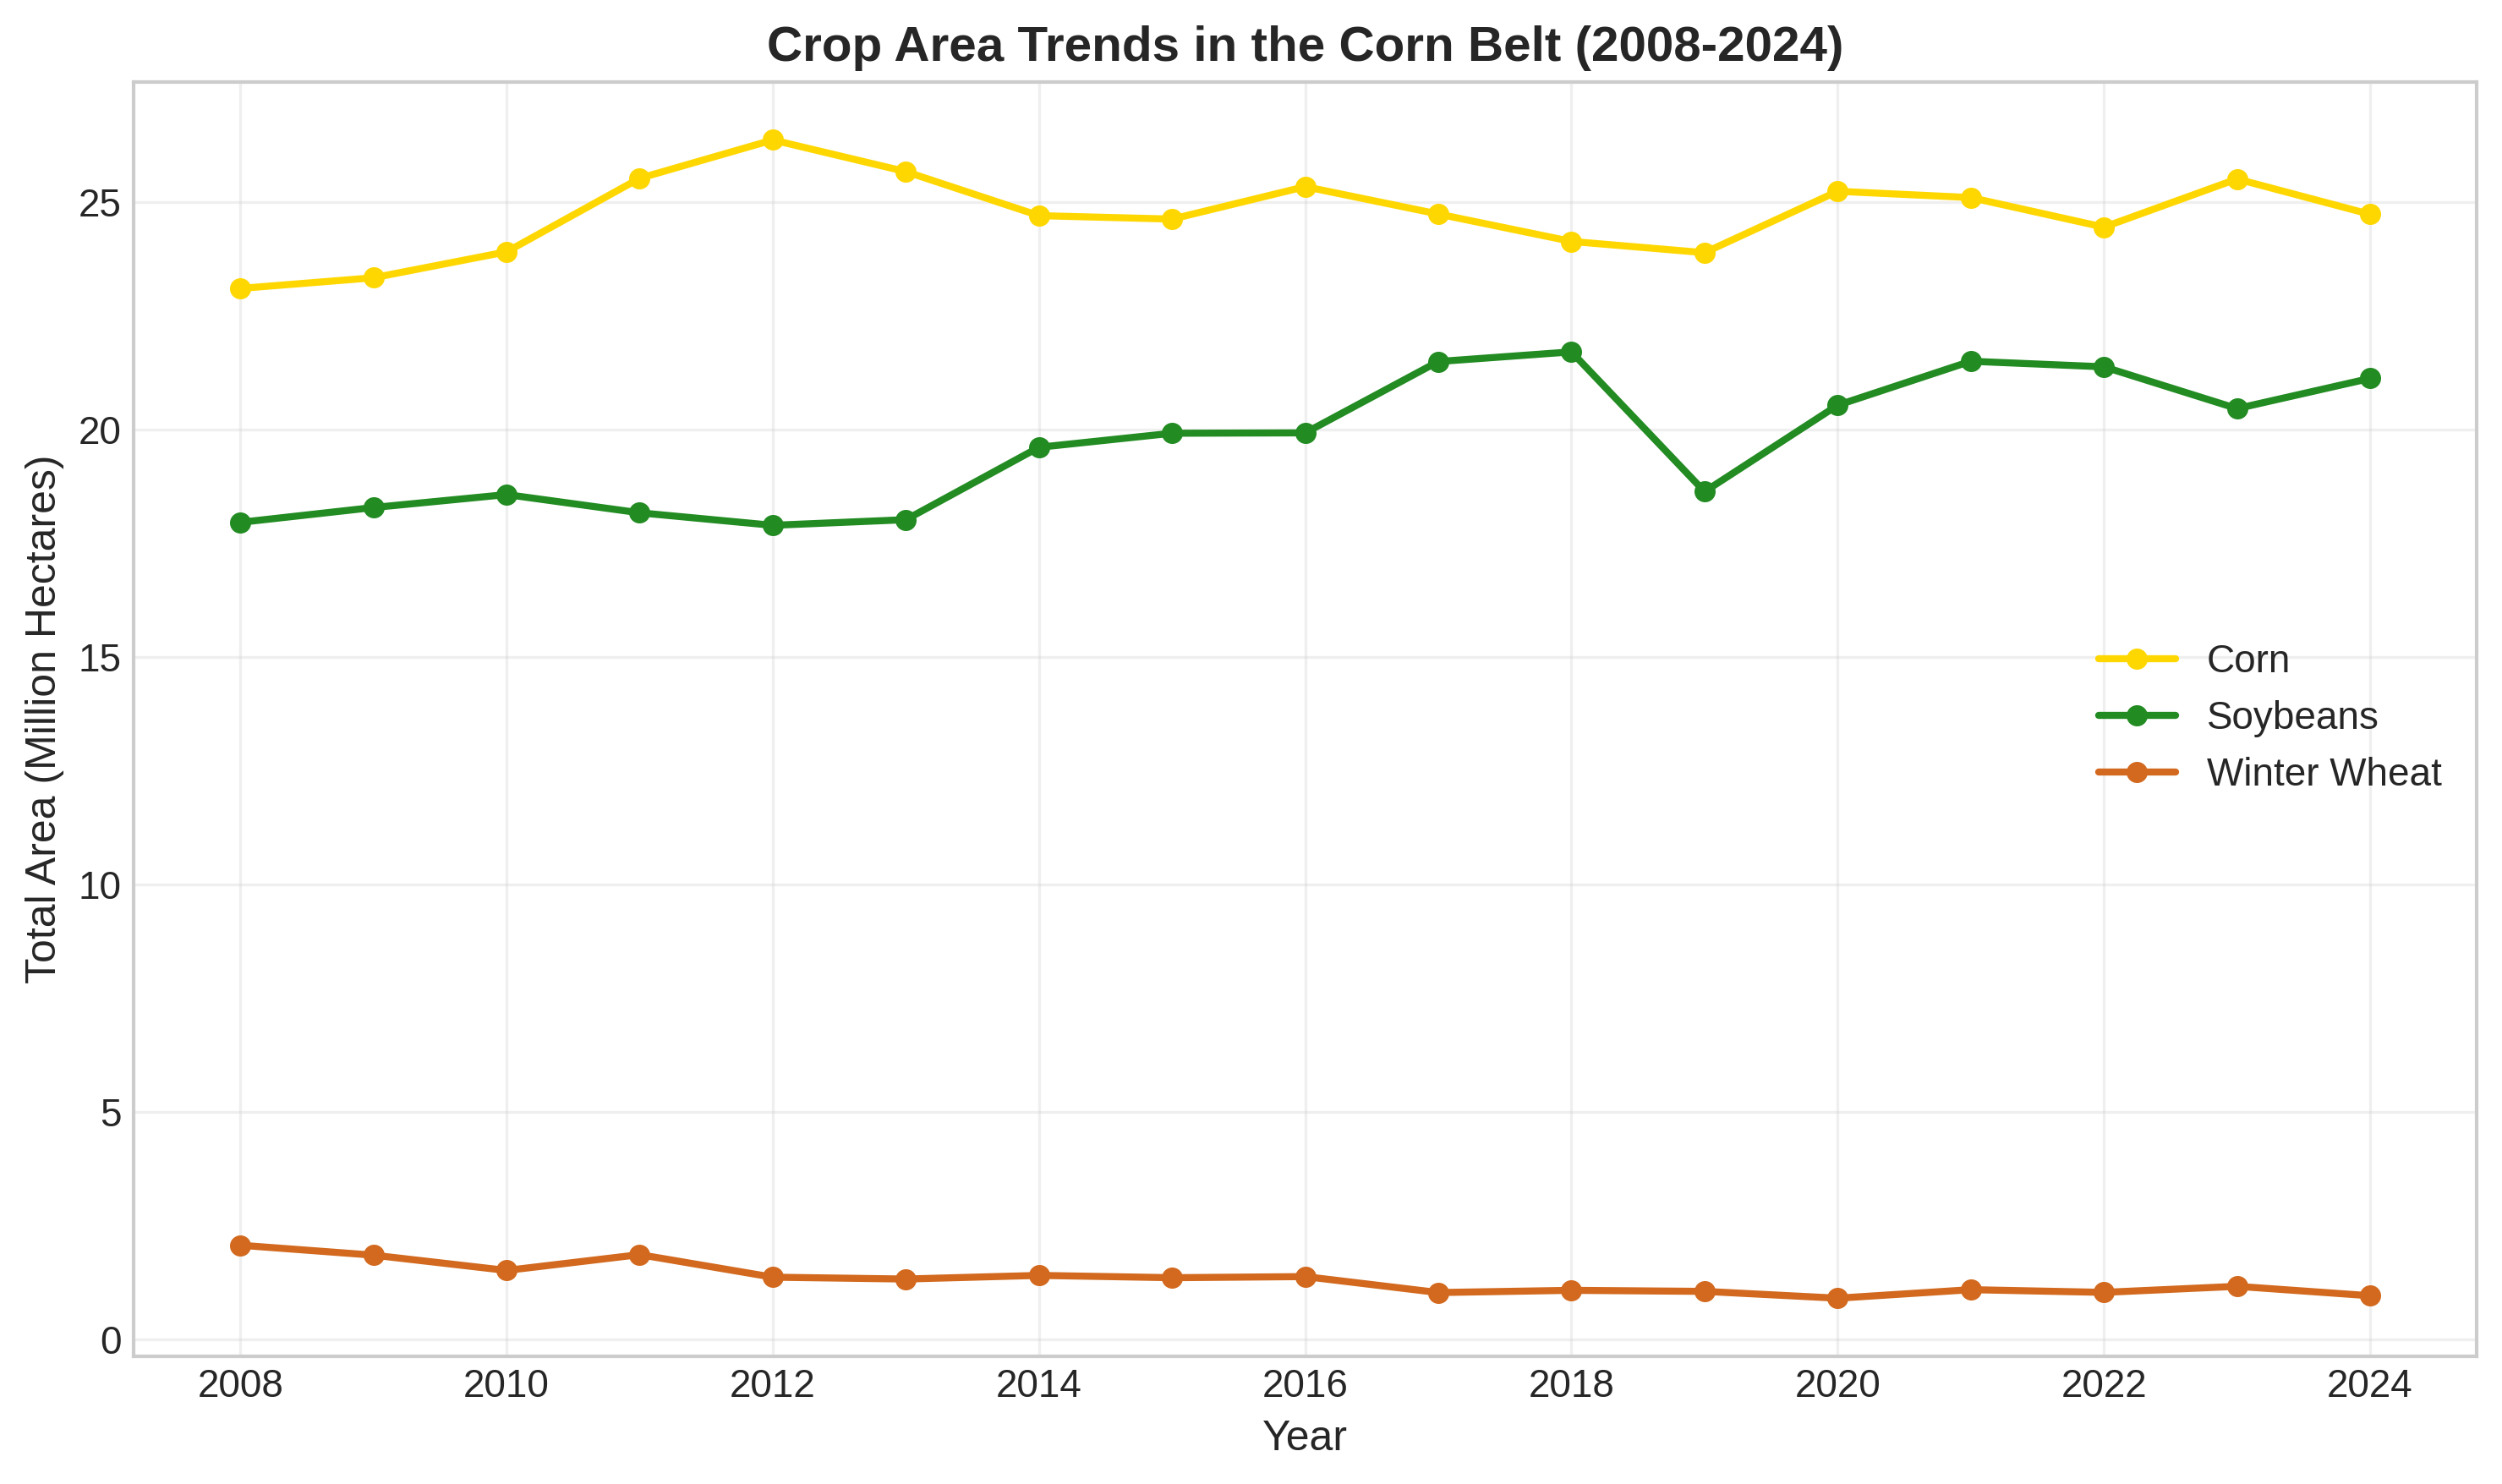
\includegraphics[width=0.9\textwidth]{figures/fig5_crop_areas_time.png}
\caption{Total crop area trends in the Corn Belt (2008--2024). Corn and soybean areas show inverse relationships, reflecting rotation dynamics and market responses.}
\label{fig:areas_time}
\end{figure}

\begin{figure}[H]
\centering
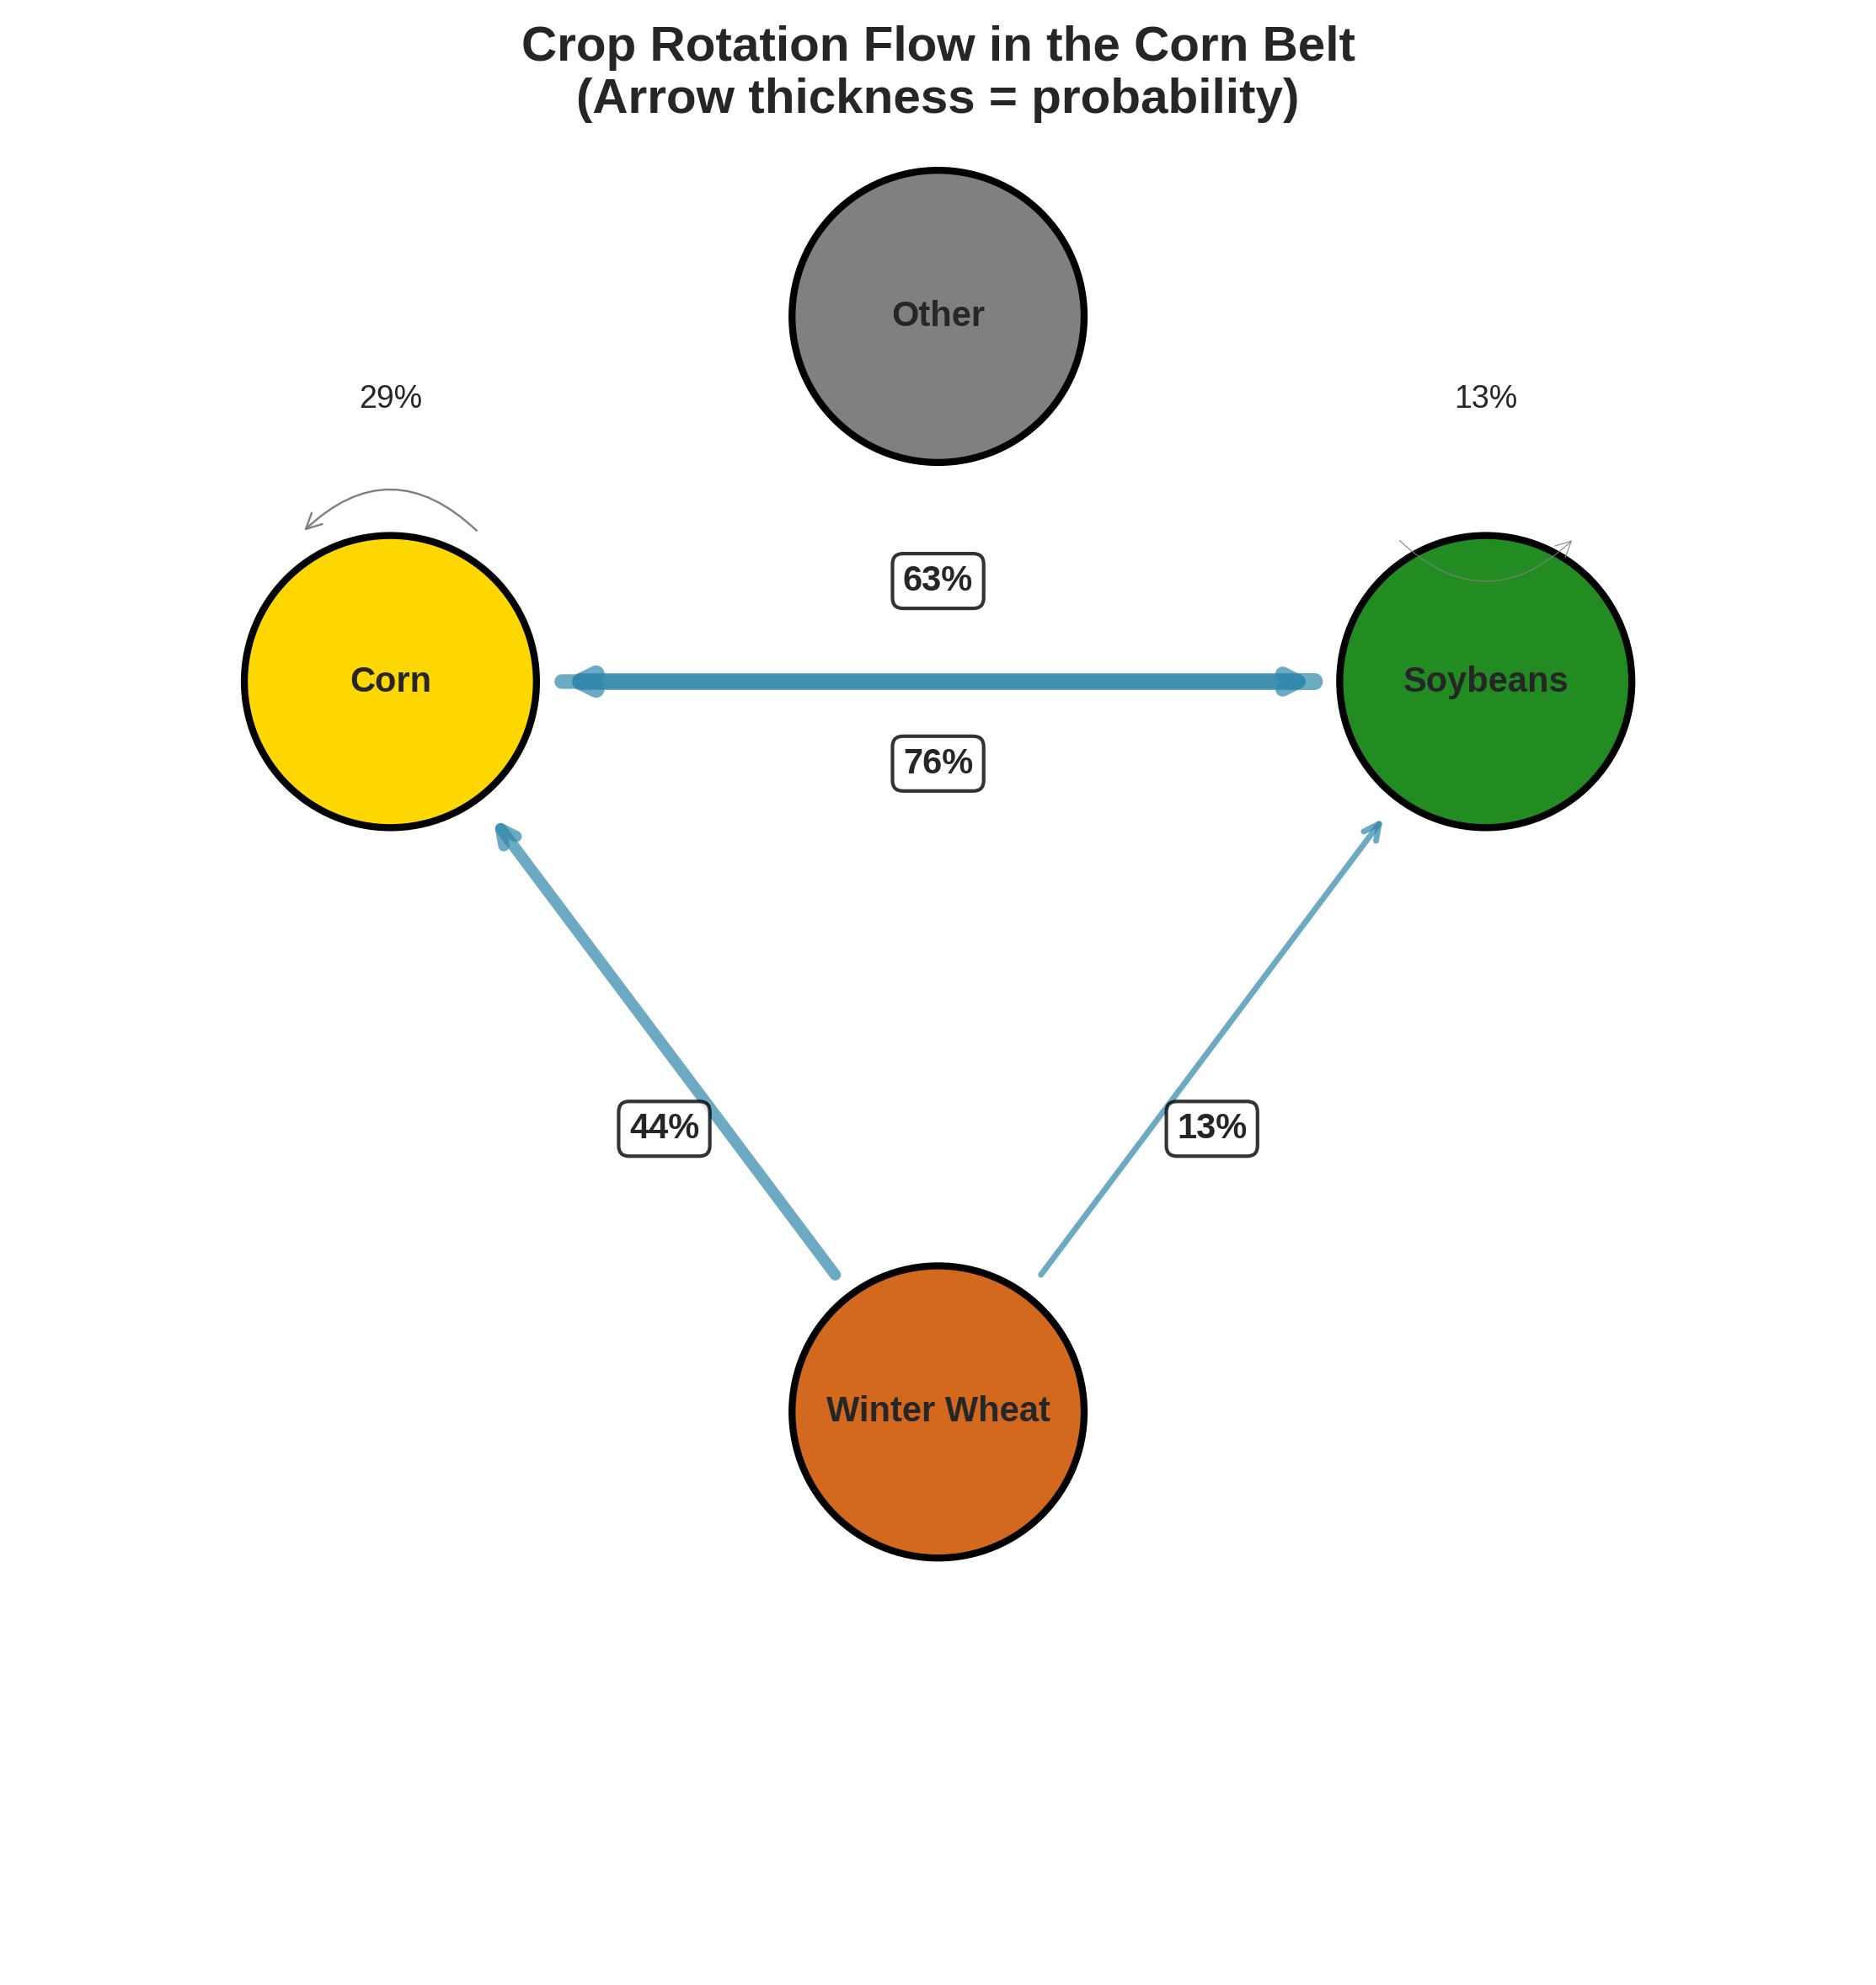
\includegraphics[width=0.8\textwidth]{figures/fig6_rotation_flow.png}
\caption{Schematic flow diagram of crop rotation in the Corn Belt. Arrow thickness represents transition probability. The bidirectional corn-soybean flow dominates.}
\label{fig:flow}
\end{figure}

\end{document}
